% The manuscript; collapse-without-rotation.pdf beside it is this file built with pdflatex, run three times
% (sh tools/paper-build.sh collapse-without-rotation in the GENChase repository).
% The figure is figures/phase-diagram.pdf, written by ../code/plot_phase_diagram.py.
% Status: DRAFT (2026-09-25). Not peer reviewed.
\documentclass[11pt]{article}
\usepackage[letterpaper,margin=1in]{geometry}
\usepackage[T1]{fontenc}
\usepackage{lmodern}
\usepackage{amsmath,amssymb,amsthm}
\usepackage{graphicx}
\usepackage{array}
\usepackage{booktabs}
\usepackage{longtable}
\usepackage{microtype}
\usepackage[hidelinks]{hyperref}

\hypersetup{
  pdftitle={Point-Vortex Collapse Without Rotation: A Cluster Mechanism, a Phase Diagram and a Continuum Limit},
  pdfauthor={Chase Hendrick}}

\newtheorem{theorem}{Theorem}
\newtheorem{lemma}{Lemma}
\newtheorem{proposition}{Proposition}
\newtheorem{corollary}{Corollary}
\theoremstyle{definition}
\newtheorem{remark}{Remark}

\renewcommand{\topfraction}{0.9}
\renewcommand{\textfraction}{0.1}
\renewcommand{\floatpagefraction}{0.8}
\setlength{\emergencystretch}{2em}

\newcommand{\re}{\operatorname{Re}}
\newcommand{\im}{\operatorname{Im}}
\newcommand{\C}{\mathbb{C}}
\newcommand{\Q}{\mathbb{Q}}
\newcommand{\R}{\mathbb{R}}
\newcommand{\K}{\mathcal{K}}
\newcommand{\hnu}{\widehat{\nu}}

\title{\Large\bfseries Point-Vortex Collapse Without Rotation:\\ A Cluster Mechanism, a Phase Diagram and a Continuum Limit}
\author{Chase Hendrick\\[0.2em] {\small Independent Researcher}\\ {\small\href{mailto:chasewhendrick@gmail.com}{\texttt{chasewhendrick@gmail.com}}}\\ {\small ORCID \href{https://orcid.org/0009-0002-9754-6087}{0009-0002-9754-6087}}}
\date{\small Draft of 25 September 2026. Not peer reviewed.}

\begin{document}
\maketitle

\begin{abstract}
In a self-similar collapse of point vortices the configuration turns through the angle $P$ while the square of its size decreases by the factor $e$. A companion paper proved that $P > \sqrt{3}/2$ for three Euler vortices, that the same constant is the limit for a strong vortex carrying weak tight pairs of opposite sign, and, with computer-assisted proofs, that eleven vortices in the $\alpha = 2$ model and sixty in the surface quasi-geostrophic (SQG) model can collapse without rotating at all. We first show that the constant $\sqrt{3}/2$ belongs to a larger class: a strong Euler vortex carrying any number of weak tight clusters, of any sizes and signs, has $P \ge \sqrt{3}/2 - o(1)$ as the clusters weaken. If $P$ stays bounded, every cluster is close to a translating relative equilibrium whose net circulation is half the sum of the squares of its circulations, measured in units of the strong one; a single isolated weak vortex forces $P$ to grow like the inverse of the weak circulations, with an explicit constant. In particular no such configuration collapses without rotation, whatever the number of vortices. We prove that a weak triple of signs $(+,+,-)$ beside a positive strong vortex gives collapses with $P$ below $\sqrt{3}/2$ by an amount proportional to the weak circulations, so that $\sqrt{3}/2$ is a limit and not a bound at a fixed strength, and that the constant cannot be increased for any number of weak vortices; a formal expansion, confirmed by high-precision numerical collapses computed at fifty digits, extends the first-order term to clusters of any size and explains why four vortices are the first to go below $\sqrt{3}/2$. We then map, numerically, the least $\alpha$ at which $N$ vortices can collapse without rotation along two families: the least $N$ is $5$, $6$, $8$, $11$, $17$, $29$ and $60$ for $\alpha = 6$, $4$, $3$, $2$, $1.5$, $1.2$ and $1$, and fits of the thresholds give a positive limit between $0.66$ and $0.80$, while fits forced to the Euler value $0$ are much worse. No self-similar collapse with nonzero total circulation is mirror symmetric; numerically, the two certified collapses without rotation are linearly unstable, with $8$ and $57$ unstable modes, and perturbed motions leave them without turning. Finally, numerically, the Euler minimizers of the companion paper approach a continuum of two point vortices and a positive vortex sheet, a kind of collapse that O'Neil found with point vortices approximating the sheet; with a density that vanishes like a square root at the tips of the sheet, the winding has a local minimum along a one-parameter family of such continua, $P_\infty = 0.47736353369161202484\ldots$, stable to forty digits if the observed exponential convergence persists, which agrees with the extrapolation of the finite family.

\medskip
\noindent\textbf{Keywords:} point vortices; vortex collapse; self-similar motion; relative equilibria; surface quasi-geostrophic equation; vortex sheet.\\
\textbf{MSC 2020:} 76B47, 37N10, 76U60.
\end{abstract}

\section{Introduction}

Three point vortices can collapse onto a point in finite time, keeping their shape while they shrink and turn; this was found by Gr\"obli (see \cite[p.~17, Fig.~3]{art1992} for the history), and the similarity solution for any number of vortices was written by Kimura \cite[Sect.~3.1]{kimura1987} and, with explicit examples, by Demina and Kudryashov \cite{dk2014}. In such a collapse every vortex runs a logarithmic spiral about the collision point, and the number $P$, the angle through which the configuration turns while the square of its size decreases by the factor $e$, measures how tightly the spirals wind. The companion paper \cite{mw2026} studies the least value of $P$. For three Euler vortices it proves $P > \sqrt{3}/2$, sharply, and in the $\alpha$-models, where a vortex induces the velocity $\Gamma r^{-\alpha-1}/(2\pi)$, it proves $P > \sqrt{3 + \alpha}/(2 + \alpha)$ for three vortices; it shows that the constant $\sqrt{3}/2$ is also the limit for a strong vortex carrying weak, tight pairs of opposite sign \cite[Theorem~3]{mw2026}; and with computer-assisted proofs it shows that the bound fails for four or more Euler vortices and that eleven vortices in the $\alpha = 2$ model and sixty in the SQG model ($\alpha = 1$) can collapse without rotating, every vortex running straight into the collision point \cite[Theorems~4, 5]{mw2026}.

This paper takes up three questions that the companion paper leaves open.

\emph{Why is $\sqrt{3}/2$ the limit for so many configurations, and when can it be beaten?} In Section~\ref{sec:clusters} we replace the pairs of \cite[Theorem~3]{mw2026} by weak tight clusters of any size and signs (Theorem~\ref{thm:clusters}). The bound $\sqrt{3}/2 - o(1)$ survives, and the proof shows what a cluster must look like in a collapse with bounded $P$: a translating relative equilibrium of the cluster's own vortices, carrying the net circulation $(1/(2\Gamma_0))\sum_k \Gamma_k^2$, whose self-induced translation makes an angle of $60^\circ$, at equal speed, with the motion induced by the strong vortex when $P$ is near $\sqrt{3}/2$. Consequently no configuration in this regime collapses without rotation, for any number of vortices (Corollary~\ref{cor:norot}). For a single weak triple we prove the next order (Theorem~\ref{thm:triple}): along a family of collapses $P = \sqrt{3}/2 + (2\sqrt{3}\,g_1g_2g_3/S)\gamma + O(\gamma^2)$, where $\gamma g_k$ are the weak circulations, with $\sum_k g_k = 0$ and one of them corrected at order $\gamma^2$, and $S = \sum_k g_k^2$, so for signs $(+,+,-)$ the constant is undershot at every small strength, and it is sharp for three weak vortices too (Corollary~\ref{cor:triple}). A formal next-order expansion for several clusters, which we confirm numerically but do not prove, shows that at a small fixed strength of the clusters $P$ goes below $\sqrt{3}/2$ when every cluster has a positive coefficient of order $\gamma$ in that expansion, as a triple of signs $(+,+,-)$ beside a positive strong vortex has and a pair never has; this is why four vortices are the first to go below $\sqrt{3}/2$.

\emph{Where do collapses without rotation live?} In Section~\ref{sec:phase} we compute, numerically, the least $\alpha$ at which $N$ vortices can collapse without rotation along two families, for $N$ up to $73$ and $79$. The thresholds decrease with $N$ but extrapolate to a positive limit, between $0.66$ and $0.80$ depending on the fit; fits that force the Euler value $0$ are much worse. This is evidence, along these families only, that Euler vortices do not collapse without rotation.

\emph{What do these collapses look like, and are they robust?} In Section~\ref{sec:structure} we prove that no self-similar collapse with nonzero total circulation is mirror symmetric (Proposition~\ref{prop:mirror}), describe numerically the nine-parameter family of collapses without rotation of eleven vortices at $\alpha = 2$, and show numerically that both certified collapses without rotation are linearly unstable, with perturbed motions that leave the collapse without having turned. In Section~\ref{sec:continuum} we compute the continuum limit of the Euler minimizers of \cite[Sect.~7]{mw2026}: two point vortices and a positive vortex sheet in self-similar collapse, of the kind O'Neil found with point vortices approximating the sheet \cite{oneil2010}, whose winding has a local minimum along a one-parameter family that agrees with the extrapolation of the finite family. Section~\ref{sec:numerics} lists the programs that check every statement, Section~\ref{sec:discussion} discusses the literature, and Section~\ref{sec:open} lists open problems.

Theorems~\ref{thm:clusters}, \ref{thm:triple} and~\ref{thm:cluster}, Lemma~\ref{lem:grow}, Corollaries~\ref{cor:norot}, \ref{cor:triple} and~\ref{cor:alln} and Proposition~\ref{prop:mirror} are proved; the first-order coefficient in Theorem~\ref{thm:triple} is computed exactly by computer algebra. Everything in Sections~\ref{sec:phase}, \ref{sec:family}, \ref{sec:stability} and~\ref{sec:continuum}, and the expansion of Section~\ref{sec:formal} beyond one triple, is numerical, computed in binary64 or in high-precision arithmetic but not in interval arithmetic, and is labelled as such.

\section{Setting}\label{sec:setting}

\subsection{Self-similar collapse and the winding number}

In the $\alpha$-models point vortices at positions $z_j \in \C$ with real circulations $\Gamma_j$ move by
\begin{equation}\label{eq:alpha}
  \frac{dz_j}{dt} = \frac{i}{2\pi} \sum_{k \ne j} \Gamma_k \frac{z_j - z_k}{|z_j - z_k|^{\alpha + 2}},
\end{equation}
so that a vortex of circulation $\Gamma$ induces the speed $|\Gamma| r^{-\alpha-1}/(2\pi)$ at distance $r$; $\alpha = 0$ is the Euler equation and $\alpha = 1$ is SQG, and we use the conventions of \cite[Sect.~2]{mw2026}. For $\alpha = 0$ we write the law as
\begin{equation}\label{eq:bs}
  \overline{\dot z_j} = \frac{1}{2\pi i} \sum_{k \ne j} \frac{\Gamma_k}{z_j - z_k}.
\end{equation}
Suppose $\sum_j \Gamma_j \ne 0$ and let $z_c = \sum_j \Gamma_j z_j/\sum_j \Gamma_j$ be the center of vorticity. If $\dot z_j = \kappa(z_j - z_c)$ for all $j$ at one instant, with $\kappa \in \C$, the motion is self-similar, and it is a collapse when $\re\kappa < 0$ \cite[Sect.~2]{mw2026}; the vortices then collide at $z_c$ at a finite time, every vortex moves on a logarithmic spiral about $z_c$, and the number
\begin{equation}\label{eq:P}
  P = \frac{|\im\kappa|}{-2\re\kappa}
\end{equation}
is the angle through which the configuration turns while the square of its size decreases by the factor $e$ \cite[Eq.~(4)]{mw2026}. A collapse is \emph{without rotation} when $\kappa$ is real, that is, $P = 0$: then every vortex moves on a straight line into the collision point. For the Euler law it is convenient to write
\begin{equation}\label{eq:Lambda}
  \Lambda = 2\pi i\,\overline{\kappa}, \qquad \re\Lambda = 2\pi\im\kappa, \qquad \im\Lambda = 2\pi\re\kappa, \qquad P = \frac{|\re\Lambda|}{-2\im\Lambda},
\end{equation}
so that a self-similar Euler configuration satisfies $\sum_{k \ne j} \Gamma_k/(z_j - z_k) = \Lambda\,\overline{(z_j - z_c)}$ for every $j$, and it collapses when $\im\Lambda < 0$.

Two classical necessary conditions constrain every self-similar collapse: the angular impulse $\sum_j \Gamma_j |z_j - z_c|^2$ is conserved and proportional to the square of the size, so it vanishes; and the Hamiltonian is conserved while it scales with the size, which for $\alpha = 0$ forces $\sum_{j<k} \Gamma_j\Gamma_k = 0$ and for $\alpha \ne 0$ forces $\sum_{j<k} \Gamma_j\Gamma_k |z_j - z_k|^{-\alpha} = 0$ \cite[Sect.~2, Lemma~1, Sect.~7]{mw2026}, \cite{dk2014}. Once translations, rotations and the scalings of lengths and circulations are divided out, the self-similar collapses of $N$ vortices form, where their equations are independent, a manifold of dimension $N - 1$ \cite[Sect.~7]{mw2026}, and those without rotation a manifold of dimension $N - 2$ at fixed $\alpha$, or $N - 1$ when $\alpha$ is free.

\subsection{What the companion paper proves}

For three Euler vortices every self-similar collapse has $P > \sqrt{3}/2$, and the constant is approached as one circulation tends to zero \cite[Theorem~1, Corollary~1]{mw2026}; for three vortices in the $\alpha$-models, $P > \sqrt{3 + \alpha}/(2 + \alpha)$ for every $\alpha > -2$ \cite[Theorem~2]{mw2026}, so three vortices never collapse without rotation. For a strong vortex carrying $m$ weak, tight pairs of opposite sign, with pair circulations of order $\gamma$, $P \ge \sqrt{3}/2 - o(1)$ as $\gamma \to 0$, and $P$ is close to $\sqrt{3}/2$ only when every pair is tilted by $60^\circ$ from the direction away from the strong vortex \cite[Theorem~3]{mw2026}; for $\gamma$ below a threshold that is not explicit the bound is strict, $P \ge \sqrt{3}/2 + (\sqrt{3}/8)c^2\gamma^2$ \cite[Proposition~4]{mw2026}. Computer-assisted proofs show that four, five and six Euler vortices collapse with $P < \sqrt{3}/2$, with strict local minima $0.7978967838\ldots$, $0.7448144569\ldots$ and $0.7136801485\ldots$ \cite[Theorem~4]{mw2026}, and that eleven vortices at $\alpha = 2$ and sixty SQG vortices collapse without rotation, in families of dimension $9$ and $58$ \cite[Theorem~5]{mw2026}. Numerically, a two-arm family of Euler minimizers reaches $P = 0.4793959201\ldots$ at $N = 603$ \cite[Sect.~7]{mw2026}. Earlier, O'Neil's point-vortex approximations of collapsing vortex sheets \cite[Fig.~3]{oneil2010} were already self-similar Euler collapses of about a hundred vortices with $P = 1/2$ (Section~\ref{sec:continuum}). No Euler collapse without rotation is known; for $\alpha = 0$ a collapse with $\kappa$ real is the same as a relative equilibrium of the imaginary circulations $i\Gamma_j$ \cite[Sect.~10]{mw2026}.

\section{A strong vortex with weak tight clusters}\label{sec:clusters}

In this section the vortices obey the Euler law \eqref{eq:bs}.

\subsection{The class and the theorem}

Let $n \ge 1$ and $0 < c \le 1$. The class $\K(n, c)$ consists of the configurations of $1 + n$ point vortices with circulation $1$ at the origin and circulations $\Gamma_k = \gamma g_k$ at $z_k$, $k = 1, \ldots, n$, where $\gamma > 0$ and $c \le |g_k| \le 1/c$, the signs of the $g_k$ being arbitrary, together with a partition of $\{1, \ldots, n\}$ into \emph{clusters} $C$ and points $Z_C \in \C$ such that
\begin{equation}\label{eq:class}
  c \le |Z_C| \le \frac{1}{c}, \quad |Z_C - Z_D| \ge c \ (C \ne D), \quad |z_k - Z_C| \le \frac{\gamma}{c} \ (k \in C), \quad |z_k - z_l| \ge c\gamma \ (k \ne l \in C).
\end{equation}
A cluster may consist of a single vortex. For $k \in C$ we write $\zeta_k = (z_k - Z_C)/\gamma$, so that $|\zeta_k| \le 1/c$ and $|\zeta_k - \zeta_l| \ge c$, and
\[
  G_C = \sum_{k \in C} g_k, \quad D_C = \sum_{k \in C} g_k\zeta_k, \quad S_C = \sum_{k \in C} g_k^2, \quad w_k = \sum_{l \in C,\, l \ne k} \frac{g_l}{\zeta_k - \zeta_l}, \quad q_C = -\frac{2D_C}{S_C Z_C} = p_C + iy_C .
\]
Thus $\gamma G_C$ is the net circulation of $C$ and $D_C$ its dipole moment in units of $\gamma^2$, and $w_k/(2\pi i)$ is the conjugate of the velocity that the other vortices of $C$ induce at $z_k$. We measure the net circulation of a cluster by the dimensionless ratio
\[
  \hnu_C = \frac{\sum_{k \in C} \Gamma_k}{\frac{1}{2\Gamma_0}\sum_{k \in C} \Gamma_k^2} = \frac{2G_C}{\gamma S_C}, \qquad \Gamma_0 = 1 ,
\]
which does not change when all circulations are multiplied by a positive constant. The normalization is no loss of generality: a translation puts the strong vortex at the origin, a positive factor on the circulations leaves $P$ unchanged, and the map $(\Gamma_j, z_j) \mapsto (-\Gamma_j, \overline{z_j})$ maps solutions of \eqref{eq:bs} to solutions, collapses to collapses with the same $P$ \cite[Sect.~3.1]{mw2026}, and $\K(n, c)$ onto itself.

The class of \cite[Theorem~3]{mw2026}, a strong vortex with $m$ pairs $\gamma a_j$ at $Z_j$ and $-\gamma b_j$ at $W_j$ with $c \le a_j, b_j \le 1/c$, $c \le |Z_j| \le 1/c$, $c\gamma|Z_j| \le |W_j - Z_j| \le \gamma|Z_j|/c$ and $|Z_j - Z_l| \ge c$, is contained in $\K(2m, c^2)$, with the pairs as clusters and $Z_C = Z_j$; for a pair, $q_C = 2b_j(W_j - Z_j)/(\gamma(a_j^2 + b_j^2)Z_j) = u_j\cdot 2a_jb_j/(a_j^2 + b_j^2)$, where $u_j = (W_j - Z_j)/(\gamma a_jZ_j)$ is the quantity of \cite{mw2026}; the factor tends to $1$ along collapses with bounded $P$, since $\hnu_C \to 1$ forces $a_j - b_j \to 0$ (part (b) below).

\begin{theorem}[A strong vortex with weak tight clusters]\label{thm:clusters}
Let $n \ge 1$ and $0 < c \le 1$, and consider the configurations of $\K(n, c)$ that collapse self-similarly, $\dot z_i = \kappa(z_i - z_c)$ for all $1 + n$ vortices with $\re\kappa < 0$.

\textup{(a)} For every $\delta > 0$ there is $\gamma_1 > 0$, depending only on $n$, $c$ and $\delta$, such that every such collapse with $\gamma < \gamma_1$ has $P > \sqrt{3}/2 - \delta$.

\textup{(b)} For every $\delta > 0$ and $\bar P > 0$ there is $\gamma_2 > 0$, depending only on $n$, $c$, $\delta$ and $\bar P$, such that every such collapse with $\gamma < \gamma_2$ and $P \le \bar P$ has, for every cluster $C$: vortices of both signs in $C$; $|p_C - 1/2| < \delta$; $|\hnu_C - 1| < \delta$; $\max_{k,\,l \in C}|w_k - w_l| < \delta$; $y_C > 0$; and
\[
  \Bigl|P - \frac{y_C^2 + 3/4}{2y_C}\Bigr| < \delta, \qquad \text{where} \quad \frac{y_C^2 + 3/4}{2y_C} = \frac{\sqrt{3}}{2} + \frac{(y_C - \sqrt{3}/2)^2}{2y_C}.
\]

\textup{(c)} For every $\delta > 0$ there are $\eta > 0$ and $\gamma_3 > 0$, depending only on $n$, $c$ and $\delta$, such that every such collapse with $\gamma < \gamma_3$ and $P < \sqrt{3}/2 + \eta$ has $|q_C - e^{i\pi/3}| < \delta$ for every cluster $C$ and $\bigl||Z_C|/|Z_D| - 1\bigr| < \delta$ for all clusters $C$ and $D$.

\textup{(d)} If some cluster consists of a single vortex, every such collapse with $\gamma \le c^3/(20n)$ has $P \ge c^3/(40n\gamma)$.

For every $n \ge 2$ the constant $\sqrt{3}/2$ in \textup{(a)} cannot be increased when $c$ is small enough (Corollary~\ref{cor:alln}); explicitly, for $n = 2$ and $c \le 1/4$, for every even $n = 2m \ge 4$ and $c \le \min(1/2, 2\sin(\pi/m))^2$, and for $n = 3$ and $c \le 1/2$ (Corollary~\ref{cor:triple}).
\end{theorem}

In words: when the clusters are weak, a collapse with bounded winding has every cluster close to a translating relative equilibrium (all the $w_k$ of the cluster nearly equal) whose net circulation, positive, is close to $(1/(2\Gamma_0))\sum_k \Gamma_k^2$; and $P$ can come close to $\sqrt{3}/2$ only if every $q_C$ is close to $e^{i\pi/3}$ and all clusters are at nearly the same distance from the strong vortex. The self-induced velocity $V_C$ of a cluster and the velocity $V_s$ induced there by the strong vortex satisfy $V_C/V_s = 1/\overline{q_C}$ in the limit (Step~4 below), so $q_C = e^{i\pi/3}$ means that the cluster translates at the speed induced by the strong vortex, at the angle $60^\circ$ to it. On $p_C = 1/2$, with $t = \arg q_C$, one has $|V_C|/|V_s| = 2\cos t$ and $P = (2 + \cos 2t)/(2\sin 2t)$.

\begin{corollary}\label{cor:norot}
For every $n \ge 1$ and $0 < c \le 1$ there is $\gamma_* > 0$ such that no configuration of $\K(n, c)$ with $\gamma < \gamma_*$ collapses self-similarly without rotation. In particular, for no number of vortices is a collapse without rotation possible in the regime of a strong vortex with sufficiently weak tight clusters.
\end{corollary}

\begin{proof}
Take $\gamma_* = \gamma_1$ of Theorem~\ref{thm:clusters}(a) with $\delta = \sqrt{3}/4$; then $P > \sqrt{3}/4 > 0$.
\end{proof}

\begin{remark}[What the class contains and excludes]\label{rem:class}
The theorem covers all of $\K(n, c)$: every partition into clusters, and clusters of every shape allowed by \eqref{eq:class}, singletons included. The proof shows more than the statement. A single vortex forces the stationary branch of Step~4, where $P \to \infty$, and (d) makes this explicit. A cluster of two or more vortices of one sign cannot occur at all in a collapse once $\gamma$ is below a constant that depends only on $n$ and $c$, since in the limit it would need $G_C^2 = S_C$, while $G_C^2 - S_C = 2\sum_{k<l} g_kg_l > 0$ (Step~4). A cluster that satisfies its own harmonic condition, $\sum_{k<l \in C} g_kg_l = 0$, could collapse by itself; such clusters fall in the stationary branch as well. Two restrictions are part of the hypotheses and cannot be dropped. Nested scales are excluded: a tight pair of size $\gamma^2$ inside a cluster of size $\gamma$ violates $|z_k - z_l| \ge c\gamma$ for every fixed $c$, and the theorem says nothing about it. And $\gamma_1$ is not uniform as $c \to 0$: the seven-vortex collapse of Demina and Kudryashov \cite[Table~1, Fig.~1a]{dk2014}, with $P = 12433/(1240\sqrt{155}) = 0.8053\ldots$ \cite[Sect.~3.2]{mw2026}, lies in $\K(6, c)$ with every weak vortex a singleton and $\gamma = c$, for every $c \le 1/3$, after its circulations are divided by the central one; so $\gamma_1(6, c, \delta) \le c$ whenever $\delta < \sqrt{3}/2 - 0.8054$.
\end{remark}

\begin{remark}[No bound at a fixed circulation]\label{rem:nobound}
For pairs, $P > \sqrt{3}/2$ at every $\gamma$ below a threshold \cite[Proposition~4]{mw2026}. For clusters there is no such statement: by Corollary~\ref{cor:triple}, a strong vortex with one triple of signs $(+,+,-)$ collapses with $P < \sqrt{3}/2$ at every small $\gamma$, so the $\delta$ in (a) cannot be removed, and $\sqrt{3}/2$ is the limit of the least $P$ as $\gamma \to 0$, not a lower bound at a fixed $\gamma$. The collapses of Table~\ref{tab:clusters}, computed at fifty digits, show the same for other arrangements at $\gamma = 10^{-2}$, $10^{-3}$ and $10^{-4}$ (numerical).
\end{remark}

\begin{remark}[The net circulation and the classical condition]\label{rem:harmonic}
With one cluster, the necessary condition $\sum_{i<j}\Gamma_i\Gamma_j = 0$ reads $\gamma G_C + \gamma^2(G_C^2 - S_C)/2 = 0$, which gives exactly $\hnu_C = 1 - \gamma^2\nu_C^2/S_C$ with $\nu_C = G_C/\gamma$, so $\hnu_C = 1 - \gamma^2 S_C/4 + O(\gamma^4)$. The collapses computed in Section~\ref{sec:formal} satisfy this to $10^{-36}$. With several clusters the classical condition only fixes $\sum_C \nu_C = \sum_C S_C/2 + O(\gamma^2)$; part (b) says that each cluster separately carries the net circulation $\gamma^2 S_C/2$ in the limit.
\end{remark}

\subsection{Proof of Theorem~\ref{thm:clusters}}

We follow the proof of \cite[Theorem~3]{mw2026}. It suffices to prove three statements about a sequence of collapses in $\K(n, c)$ with $\gamma = \gamma_j \to 0$, in which we write $P_j$, $\Lambda_j$, $q_{C,j}$ and so on:
(S1) $\liminf P_j \ge \sqrt{3}/2$;
(S2) if $P_j \to \sqrt{3}/2$, then $q_{C,j} \to e^{i\pi/3}$ and $|Z_{C,j}|/|Z_{D,j}| \to 1$ for all clusters $C$ and $D$;
(S3) if $\sup_j P_j < \infty$, then for all large $j$ every cluster has vortices of both signs, and for every cluster $p_{C,j} \to 1/2$, $\hnu_{C,j} \to 1$, $\max_{k,l \in C}|w_{k,j} - w_{l,j}| \to 0$, $\liminf_j y_{C,j} > 0$ and $P_j - (y_{C,j}^2 + 3/4)/(2y_{C,j}) \to 0$.
Indeed, if (a) failed for some $\delta$ there would be a sequence with $\gamma_j \to 0$ and $P_j \le \sqrt{3}/2 - \delta$, contrary to (S1). If (c) failed for some $\delta$, there would be a sequence with $\gamma_j \to 0$ and $P_j < \sqrt{3}/2 + 1/j$ for which one of the inequalities fails for every $j$; after passing to a subsequence the partition into clusters is the same for all $j$ (there are finitely many partitions) and the failing inequality is the same, for the same clusters; by (S1), $P_j \to \sqrt{3}/2$, contrary to (S2). The same argument with $P_j \le \bar P$ reduces (b) to (S3). Part (d) is proved separately at the end.

Throughout, $\gamma \le \gamma_0 = c^3/(16n)$, which holds along a sequence with $\gamma_j \to 0$ after finitely many terms are discarded, and $O(\gamma^k)$ denotes a quantity bounded by $\gamma^k$ times a constant that depends only on $n$ and $c$. Each identity used below is a direct computation, verified exactly in \texttt{verify\_\allowbreak cluster\_\allowbreak identities.py}; the remainders are checked in \texttt{verify\_\allowbreak cluster\_\allowbreak remainders.py} (Section~\ref{sec:numerics}).

\emph{Step 1: a priori bounds.} Since $\gamma/c \le c^2/16$, every $z_k$ with $k \in C$ lies within $c/16$ of $Z_C$, so $c/2 \le |z_k| \le 2/c$, and a vortex of $C$ and one of $D \ne C$ are at distance at least $c - 2\gamma/c \ge c/2$. The total circulation $1 + \gamma\sum_k g_k$ lies in $[1/2, 3/2]$, so $|z_c| \le 2\gamma\sum_k |g_k||z_k| \le 4n\gamma/c^2 \le c/4$. For $k \in C$ let $E_C(z) = \sum_{l \notin C} \gamma g_l/(z - z_l)$, the field of the weak vortices outside $C$; it is holomorphic on the disc $|z - Z_C| \le c/4$, where every $z_l$, $l \notin C$, is at distance at least $c/2$, so there $|E_C| \le 2n\gamma/c^2$, and $E_C'$ and $E_C''$ are also $O(\gamma)$. Moreover $|w_k| \le n/c^2$. The equation $\dot z_k = \kappa(z_k - z_c)$ at a weak vortex $k \in C$ reads, by \eqref{eq:bs} and \eqref{eq:Lambda},
\begin{equation}\label{eq:weak}
  \Lambda\,\overline{(z_k - z_c)} = \frac{1}{z_k} + w_k + E_C(z_k),
\end{equation}
since the vortices of $C$ other than $k$ contribute $\sum_{l \in C,\, l \ne k} \gamma g_l/(\gamma(\zeta_k - \zeta_l)) = w_k$. Its right side is at most $2/c + n/c^2 + 2n\gamma/c^2 \le 4n/c^2$ in absolute value and $|z_k - z_c| \ge c/4$, so $|\Lambda| \le 16n/c^3$.

\emph{Step 2: the weighted sums.} Put
\[
  T_C = \Lambda\,\overline{(Z_C - z_c)} - \frac{1}{Z_C} - E_C(Z_C).
\]
Since $z_k = Z_C + \gamma\zeta_k$, \eqref{eq:weak} gives
\begin{equation}\label{eq:W}
  w_k - T_C = \gamma\Lambda\,\overline{\zeta_k} + \Bigl(\frac{1}{Z_C} - \frac{1}{z_k}\Bigr) + \bigl(E_C(Z_C) - E_C(z_k)\bigr) = O(\gamma), \qquad k \in C.
\end{equation}
The internal field satisfies two classical identities, obtained by symmetrizing the double sums:
\[
  \text{(I1)}\quad \sum_{k \in C} g_kw_k = 0, \qquad \text{(I2)}\quad \sum_{k \in C} g_k\zeta_kw_k = \frac{1}{2}\sum_{k \ne l} g_kg_l = \frac{G_C^2 - S_C}{2}.
\]
Multiply \eqref{eq:weak} by $g_k$ and sum over $k \in C$. With the exact expansion $\sum_k g_k/z_k = G_C/Z_C - \gamma D_C/Z_C^2 + \gamma^2\sum_k g_k\zeta_k^2/(Z_C^2z_k)$, the Taylor expansion $\sum_k g_kE_C(z_k) = G_CE_C(Z_C) + \gamma D_CE_C'(Z_C) + O(\gamma^3)$ and (I1), this gives
\begin{equation}\label{eq:A}
  G_C\,T_C = -\gamma\Bigl(\Lambda\,\overline{D_C} + \frac{D_C}{Z_C^2}\Bigr) + O(\gamma^2).
\end{equation}
Multiply \eqref{eq:weak} by $g_k\zeta_k$ and sum. With $\sum_k g_k\zeta_k/z_k = D_C/Z_C + O(\gamma)$, $\sum_k g_k\zeta_kE_C(z_k) = D_CE_C(Z_C) + O(\gamma^2)$, the term $\gamma\Lambda\sum_k g_k|\zeta_k|^2 = O(\gamma)$ and (I2),
\begin{equation}\label{eq:B}
  D_C\,T_C = \frac{G_C^2 - S_C}{2} + O(\gamma).
\end{equation}

\emph{Step 3: limits.} Along the sequence, $\Lambda_j$ is bounded, and so are $g_{k,j}$, $\zeta_{k,j}$ and $Z_{C,j}$; every subsequence therefore has a further subsequence along which the partition into clusters is fixed and $\Lambda_j \to \Lambda^*$, $g_{k,j} \to g_k^*$, $\zeta_{k,j} \to \zeta_k^*$ and $Z_{C,j} \to Z_C^*$, with $c \le |g_k^*| \le 1/c$, $c \le |Z_C^*| \le 1/c$, $|Z_C^* - Z_D^*| \ge c$ and $|\zeta_k^* - \zeta_l^*| \ge c$. We pass to such a subsequence. Since $\im\Lambda_j = 2\pi\re\kappa_j < 0$, $\im\Lambda^* \le 0$. By Step~1, $z_{c,j} \to 0$ and $E_C(Z_C) \to 0$, so $T_{C,j} \to T_C^* = \Lambda^*\overline{Z_C^*} - 1/Z_C^*$, and $G_C$, $D_C$, $S_C$ converge to $G_C^*$, $D_C^*$ and $S_C^* \ge c^2$. By \eqref{eq:A} and \eqref{eq:B},
\begin{equation}\label{eq:limit}
  G_C^*\,T_C^* = 0, \qquad D_C^*\,T_C^* = \frac{G_C^{*2} - S_C^*}{2} \qquad \text{for every cluster } C.
\end{equation}

\emph{Step 4: the two branches.} \emph{The stationary branch: some $T_C^* = 0$.} Then $\Lambda^*\overline{Z_C^*} = 1/Z_C^*$, so $\Lambda^* = 1/|Z_C^*|^2$ is real and positive; since $\re\Lambda_j \to \Lambda^* > 0$ and $\im\Lambda_j \to 0$ with $\im\Lambda_j < 0$, \eqref{eq:Lambda} gives $P_j \to \infty$. In this branch the clusters $C$ with $T_C^* = 0$ satisfy $G_C^{*2} = S_C^*$ by \eqref{eq:limit}: they have their own harmonic condition in the limit, and a single vortex, for which $G_C^2 = S_C$ always, belongs here. The other clusters satisfy $G_C^* = 0$.

\emph{The translating branch: every $T_C^* \ne 0$.} Then $G_C^* = 0$ for every $C$ by \eqref{eq:limit}, so every cluster has at least two vortices and vortices of both signs, and $D_C^* = -S_C^*/(2T_C^*) \ne 0$; in particular $D_C$ does not tend to $0$. (If $D_C^* = 0$ for some $C$, then \eqref{eq:limit} gives $G_C^{*2} = S_C^* \ge c^2$, so $G_C^* \ne 0$ and $T_C^* = 0$: the stationary branch.) For large $j$, $|T_{C,j}| \ge |T_C^*|/2$, so \eqref{eq:A} gives $G_{C,j} = O(\gamma_j)$ and
\[
  \nu_{C,j} = \frac{G_{C,j}}{\gamma_j} = -\frac{\Lambda_j\overline{D_{C,j}} + D_{C,j}/Z_{C,j}^2}{T_{C,j}} + O(\gamma_j) \;\to\; \nu_C^* = -\frac{\Lambda^*\overline{D_C^*} + D_C^*/Z_C^{*2}}{T_C^*}.
\]
Put $q_C^* = 1/(T_C^*Z_C^*) = p_C^* + iy_C^*$. Since $T_C^*Z_C^* = \Lambda^*|Z_C^*|^2 - 1$ and $D_C^* = -(S_C^*/2)\,q_C^*Z_C^*$,
\begin{equation}\label{eq:trans}
  \Lambda^*|Z_C^*|^2 = 1 + \frac{1}{q_C^*}, \qquad q_{C,j} = -\frac{2D_{C,j}}{S_{C,j}Z_{C,j}} \to q_C^*,
\end{equation}
and a direct computation gives
\begin{equation}\label{eq:nu}
  \nu_C^* = \frac{S_C^*}{2}\bigl(|q_C^*|^2 + \overline{q_C^*} + q_C^{*2}\bigr) = \frac{S_C^*}{2}\Bigl(2p_C^{*2} + p_C^* + iy_C^*(2p_C^* - 1)\Bigr).
\end{equation}
The $\nu_{C,j}$ are real, so $y_C^*(2p_C^* - 1) = 0$ for every $C$. By \eqref{eq:trans}, $\im\Lambda^* = -y_C^*/(|q_C^*|^2|Z_C^*|^2)$ and $\re\Lambda^* = (1 + p_C^*/|q_C^*|^2)/|Z_C^*|^2$, for every $C$. The geometric meaning of $q_C^*$ follows from \eqref{eq:weak} and \eqref{eq:W}: in the limit the conjugate velocity that the cluster induces on itself is $T_C^*/(2\pi i)$, and the one induced by the strong vortex is $1/(2\pi iZ_C^*)$, so their ratio is $V_C/V_s = \overline{T_C^*Z_C^*} = 1/\overline{q_C^*}$.

\emph{Case A: some $y_C^* \ne 0$.} Then $\im\Lambda^* \ne 0$, hence $\im\Lambda^* < 0$, and $y_D^* > 0$ for every cluster $D$. So $p_D^* = 1/2$ and $\nu_D^* = S_D^*/2$, that is, $\hnu_{D,j} = 2\nu_{D,j}/S_{D,j} \to 1$, for every $D$; and $\re\Lambda^* > 0$. Since $P$ is a continuous function of $\Lambda$ on $\im\Lambda < 0$, $P_j$ converges to
\[
  P^* = \frac{\re\Lambda^*}{-2\im\Lambda^*} = \frac{|q_D^*|^2 + p_D^*}{2y_D^*} = \frac{y_D^{*2} + 3/4}{2y_D^*} = \frac{\sqrt{3}}{2} + \frac{(y_D^* - \sqrt{3}/2)^2}{2y_D^*} \ge \frac{\sqrt{3}}{2},
\]
the same number for every $D$. Every $y_D^*$ is therefore one of the two positive roots, $y^*$ and $3/(4y^*)$, of $y^2 - 2P^*y + 3/4$, and by \eqref{eq:trans} clusters with different roots lie at different distances from the strong vortex. If $P^* = \sqrt{3}/2$, the roots coincide, every $y_D^* = \sqrt{3}/2$ and $q_D^* = e^{i\pi/3}$, and \eqref{eq:trans} gives the same $|Z_D^*|$ for every $D$.

\emph{Case B: every $y_C^* = 0$.} Then $\Lambda^*$ is real. If $\Lambda^* \ne 0$, then $\re\Lambda_j$ is bounded away from $0$ while $\im\Lambda_j \to 0$, so $P_j \to \infty$. If $\Lambda^* = 0$, then $1 + 1/p_C^* = 0$ by \eqref{eq:trans}, so $q_C^* = -1$ and, by \eqref{eq:nu}, $\nu_C^* = S_C^*/2$ for every $C$. Here the angular impulse enters. In the translating branch $\sum_i \Gamma_iz_i = \sum_C(\gamma G_CZ_C + \gamma^2D_C) = O(\gamma^2)$, so $z_c = O(\gamma^2)$; the angular impulse $\sum_i\Gamma_i|z_i - z_c|^2 = \sum_i\Gamma_i|z_i|^2 - |z_c|^2\sum_i\Gamma_i$ vanishes, and cluster $C$ contributes $\gamma G_C|Z_C|^2 + 2\gamma^2\re(\overline{Z_C}D_C) + O(\gamma^3)$ to $\sum_i\Gamma_i|z_i|^2$. Dividing by $\gamma^2$ and passing to the limit,
\begin{equation}\label{eq:imp}
  \sum_C \bigl(\nu_C^*|Z_C^*|^2 + 2\re(\overline{Z_C^*}D_C^*)\bigr) = \sum_C \frac{S_C^*}{2}|Z_C^*|^2\bigl(2p_C^{*2} - p_C^*\bigr) = 0,
\end{equation}
where we used \eqref{eq:nu} and $D_C^* = -(S_C^*/2)\,q_C^*Z_C^*$. At $p_C^* = -1$ every term is $(3/2)S_C^*|Z_C^*|^2 > 0$, which is impossible. (In Case A, $p_C^* = 1/2$ and \eqref{eq:imp} holds term by term.)

\emph{Step 5: conclusion.} Every subsequence has a further subsequence along which either $P_j \to \infty$ or Case~A holds and $P_j \to P^* \ge \sqrt{3}/2$; this proves (S1). If $P_j \to \sqrt{3}/2$, only Case~A with $P^* = \sqrt{3}/2$ can occur, so every subsequence has a further subsequence along which $q_{C,j} \to e^{i\pi/3}$ and $|Z_{C,j}|/|Z_{D,j}| \to 1$; these limits do not depend on the subsequence, so the whole sequence converges to them, which proves (S2). If $\sup_j P_j < \infty$, only Case~A can occur, and the same argument gives $p_{C,j} \to 1/2$, $\hnu_{C,j} \to 1$ and $P_j - (y_{C,j}^2 + 3/4)/(2y_{C,j}) \to 0$; $\liminf_j y_{C,j} > 0$ because every subsequence has a further subsequence along which $y_{C,j}$ has a positive limit; for large $j$ every cluster has vortices of both signs because $G_C^* = 0$ and $|g_k^*| \ge c$; and $\max_{k,l}|w_k - w_l| \to 0$ by \eqref{eq:W}. This proves (S3). The argument for Remark~\ref{rem:class} is the same: a cluster of two or more vortices of one sign has $|G_C^*| \ge 2c$, so it can lie in neither branch, since the translating branch needs $G_C^* = 0$ and the stationary branch needs $G_C^{*2} = S_C^*$, while $G_C^{*2} - S_C^* \ge 2c^2$.

\emph{Proof of (d).} Let $k$ be the vortex of a single-vortex cluster, and let $\gamma \le c^3/(20n)$, which is below $\gamma_0$. Multiplying \eqref{eq:weak}, where now $w_k = 0$, by $z_k$ gives $\Lambda|z_k|^2(1 - \varepsilon_1) = 1 + \varepsilon_2$ with $\varepsilon_1 = \overline{z_c/z_k}$ and $\varepsilon_2 = z_kE_C(z_k)$. Now $|z_k| \ge c - \gamma/c \ge 19c/20$, the total circulation is at least $19/20$, and $|\sum_i\Gamma_iz_i| \le n\gamma(1 + \gamma)/c^2$, so $|\varepsilon_1| \le (20/19)^2(21/20)\,n\gamma/c^3 < 1.2\,n\gamma/c^3$. The other weak vortices are at distance at least $c - 2\gamma/c$ from $z_k$ and $|z_k| \le (1 + \gamma)/c$, so $|\varepsilon_2| \le (n - 1)\gamma(1 + \gamma)/(c^3(1 - 2\gamma/c^2))$, which is at most $n\gamma/c^3$ because $\gamma \le 1/(20n)$, $2\gamma/c^2 \le 1/(10n)$ and $(n - 1)(20n + 1) \le 2n(10n - 1)$. With $x = 10n\gamma/c^3 \le 1/2$ we have $|\varepsilon_1| \le 0.4x$ and $|\varepsilon_2| \le 0.1x$, hence
\[
  \bigl|\Lambda|z_k|^2 - 1\bigr| \le \frac{|\varepsilon_1| + |\varepsilon_2|}{1 - |\varepsilon_1|} \le \frac{0.5x}{1 - 0.4x} \le x,
\]
because $x - 0.5x/(1 - 0.4x) = x(5 - 4x)/(2(5 - 2x)) \ge 0$. So $\re(\Lambda|z_k|^2) \ge 1 - x$ and $|\im(\Lambda|z_k|^2)| \le x$, and \eqref{eq:Lambda} gives $P \ge (1 - x)/(2x) \ge 1/(4x) = c^3/(40n\gamma)$.

\emph{Sharpness.} The class of \cite[Theorem~3]{mw2026} lies in $\K(2m, c^2)$, and, as shown after the proof of \cite[Theorem~3]{mw2026}, the collapses of three vortices and of two rings with a central vortex \cite[Corollary~1, Proposition~3]{mw2026} lie in that class, with $m = 1$ and $c = 1/2$ and with $m \ge 2$ and $c = \min(1/2, 2\sin(\pi/m))$, and have $P \to \sqrt{3}/2$. Since $\K(n, c)$ grows as $c$ decreases, $\sqrt{3}/2$ in (a) cannot be increased for $n = 2m$ and every $c$ up to the squares of these values. For larger $c$ it can be: at $c = 1$ and $n = 2$ the weak circulations are $\pm\gamma$, the condition $\sum_{i<j}\Gamma_i\Gamma_j = 0$ has no solution with $\gamma < 2$, and no configuration with $\gamma < 2$ collapses.
\qed

For $n = 1$, part (d) gives $P \to \infty$, so (a) holds with any constant. For $n = 3$ the constant $\sqrt{3}/2$ is sharp for $c \le 1/2$, by Corollary~\ref{cor:triple}, and for every $n \ge 2$ it is sharp for small $c$, by Corollary~\ref{cor:alln}, with one cluster of $n$ weak vortices; a strong vortex with a pair and a triple ($n = 5$, two clusters) has least $P$ tending to $\sqrt{3}/2$ from above (Table~\ref{tab:clusters}; numerical).

\subsection{Beyond leading order: why four vortices go below \texorpdfstring{$\sqrt{3}/2$}{sqrt(3)/2}}\label{sec:formal}

The following expansion is formal: we carry the equations of Step~2 one order further in $\gamma$ without controlling the remainders, and we confirm the result numerically. For one triple its first-order term is proved in Section~\ref{sec:triple}. For a cluster with $G_C = O(\gamma)$ let $M_C = \sum_k g_k\zeta_k^2$, $N_C = \sum_k g_k|\zeta_k|^2$ and
\[
  J_C = N_C - \re\Bigl(\overline{M_C}\,\frac{D_C}{\overline{D_C}}\Bigr) = 2\sum_{k \in C} g_kh_k^2, \qquad e_C = \frac{\gamma J_C S_C}{2|D_C|^2},
\]
where $h_k$ is the coordinate of $\zeta_k$ perpendicular to the dipole $D_C$; $J_C$ does not depend on the point $Z_C$ from which $\zeta_k$ is measured. Measured from the point where $M_C = 0$, the next term of \eqref{eq:B} is $D_CT_C = -S_C/2 - \gamma\Lambda N_C + O(\gamma^2)$, and with $L = \Lambda|Z_C|^2$ this becomes $L = 1 + (1 + e_CL)/q_C$, so $L = (q_C + 1)/(q_C - e_C)$. Carrying \eqref{eq:A} to the same order gives $\nu_C/(S_C/2) = (|q_C|^2 + \overline{q_C} + q_C^2 - e_Cq_C)/(1 + e_C)$, which is real only if $y_C(2p_C - 1 - e_C) = 0$. On $p_C = (1 + e_C)/2$,
\[
  P = \frac{(3 + e_C)(1 - e_C)/4 + y_C^2}{2y_C(1 + e_C)} \ge \frac{\sqrt{(3 + e_C)(1 - e_C)}}{2(1 + e_C)} = \frac{\sqrt{3}}{2} - \frac{2}{\sqrt{3}}\,e_C + O(e_C^2).
\]
All clusters share $\Lambda$, so each gives such a lower bound, and the least $P$ over a family in which the cluster shapes and the directions of the clusters are fixed is, formally,
\begin{equation}\label{eq:formal}
  P_{\min} = \frac{\sqrt{3}}{2} - \frac{2}{\sqrt{3}}\min_C e_C + O(\gamma^2).
\end{equation}
For a pair both vortices lie on the axis of the dipole, so $J_C = 0$ and $e_C = 0$: there is no term of order $\gamma$, in agreement with \cite[Proposition~4]{mw2026}, where the first correction is of order $\gamma^2$ and positive. For a triple with $G_C = 0$ the translating relative equilibria we use are equilateral, and then $e_C = -3\gamma g_1g_2g_3/S_C$, so the slope in \eqref{eq:formal} is $2\sqrt{3}\,g_1g_2g_3/S_C$. With a positive strong vortex this is negative for a triple of signs $(+,+,-)$: such a triple goes below $\sqrt{3}/2$ at first order in $\gamma$, while a triple $(+,-,-)$ stays above. For the triple $g = (1, 0.6, -1.6)$ the slope is $2\sqrt{3}(-0.96)/3.92 = -0.84835\ldots$; this number belongs to that triple only.

Table~\ref{tab:clusters} compares \eqref{eq:formal} with collapses computed at fifty digits. For each arrangement the cluster shapes are translating relative equilibria of zero net circulation, the circulations of each cluster except one and the directions of the cluster centers are fixed, and the remaining unknowns (all positions, $\Lambda$ and one circulation per cluster) are found by Newton's method at fifty digits along the one-parameter family parametrized by $y$ of the binding cluster; $P_{\min}$ is the least $P$ along that family, so it is minimized over $y$ only, with the shapes and directions fixed. Every point used is accepted only after the Biot--Savart velocities \eqref{eq:bs} of all vortices, the strong one included, agree with $\kappa(z_j - z_c)$ to $10^{-40}$ relative. In every arrangement the error of the slope in \eqref{eq:formal} shrinks by a factor between $9.9$ and $10.6$ per decade of $\gamma$, which is the $O(\gamma^2)$ remainder; with a pair in the arrangement the pair binds, $\min_C e_C = 0$, and $P_{\min} > \sqrt{3}/2$.

\begin{table}[t]
\centering
\small
\renewcommand{\arraystretch}{1.15}
\begin{tabular}{@{}lrrrrr@{}}
\toprule
clusters beside a strong vortex $+1$ & $\min_C e_C/\gamma$ & slope of \eqref{eq:formal} & \multicolumn{3}{c}{$(P_{\min} - \sqrt{3}/2)/\gamma$ at $\gamma =$} \\
 & & & $10^{-2}$ & $10^{-3}$ & $10^{-4}$ \\
\midrule
pair $(0.9, -0.9)$ & $0$ & $0$ & $0.010428$ & $0.001051$ & $0.000105$ \\
triple $(1, 0.6, -1.6)$ & $0.73469$ & $-0.84835$ & $-0.79999$ & $-0.84347$ & $-0.84786$ \\
triple $(0.8, -1.3, 0.5)$ & $0.60465$ & $-0.69819$ & $-0.67852$ & $-0.69624$ & $-0.69800$ \\
quadruple $(1, 0.7, -0.5, -1.2)$ & $0.15302$ & $-0.17670$ & $-0.11027$ & $-0.17009$ & $-0.17604$ \\
quadruple $(1, 0.9, 0.8, -2.7)$ & $1.83673$ & $-2.12088$ & $-1.99482$ & $-2.10832$ & $-2.11962$ \\
pair and triple $(1, 0.6, -1.6)$ & $0$ & $0$ & $0.010580$ & $0.001002$ & $0.000098$ \\
two triples and a quadruple & $0.15302$ & $-0.17670$ & $-0.11815$ & $-0.17077$ & $-0.17611$ \\
triple $(-1, -0.6, 1.6)$ & $-0.73469$ & $0.84835$ & $0.89766$ & $0.85324$ & $0.84884$ \\
\bottomrule
\end{tabular}
\caption{The formal expansion \eqref{eq:formal} against collapses computed at fifty digits (\texttt{verify\_\allowbreak cluster\_\allowbreak collapses.py}; numerical). Cluster circulations are the $g_k$ of the cluster; $P_{\min}$ is minimized over $y$ with the cluster shapes and directions fixed. The error of the slope falls by a factor between $9.9$ and $10.6$ per decade in every row. With a pair present, $(P_{\min} - \sqrt{3}/2)/\gamma^2$ is $1.043$, $1.051$, $1.052$ (pair) and $1.058$, $1.002$, $0.983$ (pair and triple).}\label{tab:clusters}
\end{table}

This explains the structure found in \cite{mw2026}. Three vortices are a strong vortex and a pair, $e = 0$, and $P > \sqrt{3}/2$ \cite[Corollary~1]{mw2026}. The first configuration with a term of order $\gamma$ is a strong vortex with a triple, four vortices, and with signs $(+,+,-)$ that term is negative. The certified four-vortex minimum $P_4 = 0.7978967838\ldots$ of \cite[Theorem~4]{mw2026} has exactly this structure: one strong vortex and a $(+,+,-)$ triple with circulations $0.104$, $0.167$ and $-0.227$ times the strong one, whose net circulation is $0.978$ times $(1/2)\sum_k\Gamma_k^2$ (in units of the strong circulation), as Theorem~\ref{thm:clusters}(b) predicts for weak clusters. There the triple is not weak (its diameter is $0.23$ times its distance from the strong vortex), so \eqref{eq:formal} is only a qualitative guide: it predicts the sign of the effect, not the value.

\subsection{A proof for one triple}\label{sec:triple}

For a strong vortex with a single weak triple the first-order term of \eqref{eq:formal} can be proved. The limit $\gamma \to 0$ is degenerate: at $\gamma = 0$ the equations say only that the triple translates, which leaves its size and orientation free, and the condition that selects $p_C = 1/2$ appears one order later (Step~4). Dividing that combination of the equations by $\gamma$ removes the degeneracy, and the implicit function theorem applies.

\begin{theorem}[One weak triple]\label{thm:triple}
Let $g_1$, $g_2$, $g_3$ be nonzero real numbers with $g_1 + g_2 + g_3 = 0$, let $S = g_1^2 + g_2^2 + g_3^2$, let $y_0 > 0$ and $q_0 = 1/2 + iy_0$, and let $\omega = e^{2\pi i/3}$ or $\omega = e^{-2\pi i/3}$. There are $\varepsilon > 0$ and real-analytic functions $\zeta_1$, $\zeta_2$, $\zeta_3 = -\zeta_1 - \zeta_2$, $\Lambda$ and $\nu$ of $\gamma \in (-\varepsilon, \varepsilon)$, with
\[
  \zeta_k(0) = a\,\omega^k, \quad a = \frac{q_0}{3}\bigl(g_1(1 - \omega^2) + g_2(1 - \omega)\bigr), \qquad \Lambda(0) = 1 + \frac{1}{q_0}, \qquad \nu(0) = \frac{S}{2},
\]
such that for $0 < \gamma < \varepsilon$ the vortex of circulation $1$ at the origin and the vortices of circulations $\gamma g_1$, $\gamma g_2$ and $\gamma(g_3 + \gamma\nu(\gamma))$ at the points $1 + \gamma\zeta_k(\gamma)$ collapse self-similarly, with $\Lambda = \Lambda(\gamma)$ in \eqref{eq:Lambda}, and $\im(-2D/S) = y_0$, where $D$ and $S$ are computed with these circulations. Along this family $P$ is a real-analytic function of $\gamma$ with $P(0) = (y_0^2 + 3/4)/(2y_0)$, and for $y_0 = \sqrt{3}/2$
\begin{equation}\label{eq:triple}
  P(\gamma) = \frac{\sqrt{3}}{2} + \frac{2\sqrt{3}\,g_1g_2g_3}{S}\,\gamma + O(\gamma^2).
\end{equation}
\end{theorem}

The slope in \eqref{eq:triple} is the one \eqref{eq:formal} gives for an equilateral triple, $-(2/\sqrt{3})\,e_C/\gamma$ with $e_C = -3\gamma g_1g_2g_3/S$. It is also the slope of the least $P$ over $y_0$ near $\sqrt{3}/2$: the family is analytic in $(\gamma, y_0)$ jointly, since $F$ is, and at $\gamma = 0$ the function $(y_0^2 + 3/4)/(2y_0)$ has a nondegenerate minimum at $y_0 = \sqrt{3}/2$, so the minimizing $y_0$ moves by $O(\gamma)$ and changes $P$ only at order $\gamma^2$. By Theorem~\ref{thm:clusters}(b) every collapse with bounded $P$ has $P$ close to $(y_C^2 + 3/4)/(2y_C)$; for a triple, and by Theorem~\ref{thm:cluster} for any nondegenerate translating cluster, every value on that curve is attained in the limit $\gamma \to 0$.

\begin{corollary}\label{cor:triple}
Take $g = (1, 1, -2)$ and $y_0 = \sqrt{3}/2$ in Theorem~\ref{thm:triple}, so that the slope in \eqref{eq:triple} is $-2/\sqrt{3}$. For every small $\gamma > 0$ the collapse lies in $\K(3, c)$ for every $c \le 1/2$ and has $P < \sqrt{3}/2$, and $P \to \sqrt{3}/2$ as $\gamma \to 0$. Consequently, for $n = 3$ and $c \le 1/2$, the $\delta$ in Theorem~\ref{thm:clusters}(a) cannot be removed, and the constant $\sqrt{3}/2$ there cannot be increased.
\end{corollary}

\begin{proof}[Proof of Theorem~\ref{thm:triple}]
Write $\tilde g_1 = g_1$, $\tilde g_2 = g_2$, $\tilde g_3 = g_3 + \gamma\nu$, $w_k = \sum_{l \ne k}\tilde g_l/(\zeta_k - \zeta_l)$, $D = \sum_k \tilde g_k\zeta_k$ and $S = \sum_k \tilde g_k^2$. The total circulation is $1 + \gamma^2\nu$ and the center of vorticity is $z_c = \gamma^2(\nu + D)/(1 + \gamma^2\nu)$. By \eqref{eq:weak}, with no other weak vortices, the equation of the weak vortex $k$ is $E_k = 0$, where
\[
  E_k = \frac{1}{1 + \gamma\zeta_k} + w_k - \Lambda\,\overline{(1 + \gamma\zeta_k - z_c)} .
\]
The equation of the strong vortex follows from the other three, because $\sum_j \Gamma_j\bigl(\sum_{l \ne j}\Gamma_l/(z_j - z_l) - \Lambda\,\overline{(z_j - z_c)}\bigr) = 0$ identically. By (I1), $\sum_k \tilde g_kE_k = \sum_k \tilde g_k/(1 + \gamma\zeta_k) - \Lambda\sum_k \tilde g_k\overline{(1 + \gamma\zeta_k - z_c)}$, and since $\sum_k \tilde g_k = \gamma\nu$ this equals $\gamma E_0$ with
\[
  E_0 = \nu - \sum_k \frac{\tilde g_k\zeta_k}{1 + \gamma\zeta_k} - \Lambda\bigl(\nu(1 - \overline{z_c}) + \overline{D}\bigr).
\]
Since $\tilde g_3 \ne 0$ for small $\gamma$, for $\gamma \ne 0$ the configuration is self-similar exactly when $E_1 = E_2 = E_0 = 0$. The map $F = (E_1, E_2, E_0, \im(-2D/S) - y_0)$ of $x = (\zeta_1, \zeta_2, \Lambda, \nu) \in \C^3 \times \R$ and $\gamma$, with values in $\C^3 \times \R$, is real-analytic near $\gamma = 0$.

\emph{The point at $\gamma = 0$.} There the weak circulations add to zero and $E_0 = \nu - D - \Lambda(\nu + \overline{D})$. The equilateral triangle $\zeta_k = \omega^k$ with circulations of zero sum translates: $w_1 = w_2 = w_3 = (g_1(1 - \omega^2) + g_2(1 - \omega))/3$, which is not zero since $g_1 \ne 0$. As $w_k(s\zeta) = w_k(\zeta)/s$, the choice of $a$ gives $w_k = 1/q_0$ at $\zeta_k = a\omega^k$, so $E_1 = E_2 = 0$ with $\Lambda_0 = 1 + 1/q_0$, and (I2) gives $D_0 = -(S/2)q_0$. Since $1 - \overline{q_0} = q_0$, at $\nu_0 = S/2$ we get $E_0 = (S/2)\bigl(1 + q_0 - (1 + 1/q_0)q_0\bigr) = 0$, and $\im(-2D_0/S) = \im q_0 = y_0$.

\emph{The derivative at $\gamma = 0$ is invertible.} Let $(\delta\zeta, \delta\Lambda, \delta\nu)$, with $\delta\zeta = (\delta\zeta_1, \delta\zeta_2)$, be in the kernel of $D_xF$ at this point. The derivatives of $w_1$ and $w_2$ in $(\zeta_1, \zeta_2)$ are complex-linear forms $\ell_1$, $\ell_2$ on $\C^2$, and the first two components give $\ell_1(\delta\zeta) = \ell_2(\delta\zeta) = \delta\Lambda$. The form $\ell_1 - \ell_2$ vanishes on the scaling direction $\zeta^0 = (a\omega, a\omega^2)$, since $w_1 = w_2$ at every $s\zeta^0$, and it is not zero: a direct computation gives, at the unit triangle $\zeta_k = \omega^k$, $d(w_1 - w_2) = g_3(\omega^2\,d\zeta_1 - \omega\,d\zeta_2)$, and at $\zeta_k = a\omega^k$ the same form divided by $a^2$, by homogeneity; $g_3 \ne 0$. Its kernel is therefore the complex line through $\zeta^0$, so $\delta\zeta = s\zeta^0$ with $s \in \C$; by homogeneity $\delta\Lambda = \ell_1(s\zeta^0) = -s/q_0$, and $\delta D = sD_0$. The last component gives $\im(sq_0) = 0$, so $sq_0 = r$ is real. With $\delta\nu = (S/2)\mu$, the third component, $\delta\nu - \delta D - \delta\Lambda(\nu_0 + \overline{D_0}) - \Lambda_0(\delta\nu + \overline{\delta D}) = 0$, divided by $S/2$ and multiplied by $q_0$, reads
\[
  -\mu + sq_0^2 + s(1 - \overline{q_0}) + (1 + q_0)\,\overline{s}\,\overline{q_0} = -\mu + r(2q_0 + 2) = 0,
\]
whose imaginary part is $2ry_0 = 0$. Hence $r = 0$, so $s = 0$, $\delta\zeta = 0$, $\delta\Lambda = 0$ and $\mu = 0$.

\emph{Conclusion.} By the real-analytic implicit function theorem, $F = 0$ has a real-analytic solution $x(\gamma)$ through this point for small $|\gamma|$. For small $\gamma > 0$ the configuration is self-similar and $\im\Lambda(\gamma)$ is close to $\im\Lambda_0 = -y_0/|q_0|^2 < 0$, so it collapses. $P = \re\Lambda/(-2\im\Lambda)$ is real-analytic along the family, and $\re\Lambda_0 = 1 + 1/(2|q_0|^2)$ gives $P(0) = (|q_0|^2 + 1/2)/(2y_0) = (y_0^2 + 3/4)/(2y_0)$. The substitution $(\gamma, g_k, \zeta_k, \nu) \mapsto (\gamma/\lambda, \lambda g_k, \lambda\zeta_k, \lambda^2\nu)$, $\lambda \ne 0$, changes neither the configuration, nor $\Lambda$, nor $D/S$, and maps the family for $g$ to the family for $\lambda g$ with $\gamma$ replaced by $\gamma/\lambda$; with $\lambda = 1/g_1$ we may take $g_1 = 1$, the family being defined for $\gamma$ of both signs. The derivative $P'(0)$ is obtained by solving $D_xF\,x'(0) = -\partial_\gamma F$ at $\gamma = 0$. We solved this linear system exactly, over the field $\Q(t)(\omega)$ with $g = (1, t, -1 - t)$ and for both choices of $\omega$ (\texttt{verify\_\allowbreak triple\_\allowbreak branch.py}): at $y_0 = \sqrt{3}/2$ it gives $P'(0) = 2\sqrt{3}\,g_1g_2g_3/S$ identically in $t$ (and $\nu'(0) = g_3S/2$). The same program checks the closed form of $\ell_1 - \ell_2$ used above. Scaling back, $P'(0)$ is $g_1$ times this value for $g/g_1$, which is $2\sqrt{3}\,g_1g_2g_3/S$ again.
\end{proof}

\begin{proof}[Proof of Corollary~\ref{cor:triple}]
For $g = (1, 1, -2)$ we have $a = q_0$, so at $\gamma = 0$ the weak vortices are at $|\zeta_k| = 1$ with mutual distances $\sqrt{3}$, $S = 6$ and $\nu(0) = 3$, so $|\tilde g_3| = 2 - 3\gamma + O(\gamma^2)$. For small $\gamma > 0$ the conditions \eqref{eq:class} therefore hold with $c = 1/2$ and $Z_C = 1$, and they hold for every smaller $c$ as well. By \eqref{eq:triple}, $P = \sqrt{3}/2 - (2/\sqrt{3})\gamma + O(\gamma^2)$. Given $\gamma_1 > 0$, the family has members with $\gamma < \gamma_1$ and $P < \sqrt{3}/2$, so no $\gamma_1$ gives (a) with $\delta = 0$; and $P \to \sqrt{3}/2$, so no constant larger than $\sqrt{3}/2$ works in (a).
\end{proof}

The proof of Theorem~\ref{thm:triple} uses only (I1), (I2) and the nondegeneracy of the triangle, so its existence part holds for any single cluster that translates nondegenerately; the first-order coefficient in \eqref{eq:triple} we have computed only for triples. For a cluster of $m$ vortices with circulations $g_k$ we write $w_k = \sum_{l \ne k} g_l/(\zeta_k - \zeta_l)$ as before, and call a configuration $\zeta^\circ$ with distinct entries and $\sum_k\zeta^\circ_k = 0$ a \emph{nondegenerate translating cluster} if $w_1 = \cdots = w_m = 1$ at $\zeta^\circ$ and the complex-linear map $\delta\zeta \mapsto (dw_1(\delta\zeta), \ldots, dw_{m-1}(\delta\zeta))$ on $\{\delta\zeta \in \C^m: \sum_k\delta\zeta_k = 0\}$ is invertible. Such a cluster, with unit circulations $g_k$, translates with velocity $i/(2\pi)$, and $\sum_kg_k = 0$ is then forced by (I1). Since $\sum_kg_kw_k = 0$ for every configuration, $\sum_kg_k\,dw_k = 0$, so the component left out may be any $k$ with $g_k \ne 0$, and since the $w_k$ are invariant under translations, $\sum_k\delta\zeta_k = 0$ may be replaced by any other complement of the translations.

\begin{theorem}[One weak cluster]\label{thm:cluster}
Let $m \ge 2$, let $g_1, \ldots, g_m$ be nonzero real numbers, and let $\zeta^\circ$ be a nondegenerate translating cluster for them. Let $y_0 > 0$ and $q_0 = 1/2 + iy_0$. There are $\varepsilon > 0$ and real-analytic functions $\zeta_1, \ldots, \zeta_m$ with $\sum_k\zeta_k = 0$, $\Lambda$ and $\nu$ of $\gamma \in (-\varepsilon, \varepsilon)$, with $\zeta_k(0) = q_0\zeta^\circ_k$, $\Lambda(0) = 1 + 1/q_0$ and $\nu(0) = S/2$, $S = \sum_kg_k^2$, such that for $0 < |\gamma| < \varepsilon$ the vortex of circulation $1$ at the origin and the vortices of circulations $\gamma g_1, \ldots, \gamma g_{m-1}$ and $\gamma(g_m + \gamma\nu(\gamma))$ at the points $1 + \gamma\zeta_k(\gamma)$ collapse self-similarly, with $\Lambda = \Lambda(\gamma)$ in \eqref{eq:Lambda}. Along this family $P$ is a real-analytic function of $\gamma$ with $P(0) = (y_0^2 + 3/4)/(2y_0)$.
\end{theorem}

\begin{proof}
The proof of Theorem~\ref{thm:triple} applies with $m - 1$ in place of $2$. The map
\[
  F = \bigl(E_1, \ldots, E_{m-1}, E_0, \im(-2D/S) - y_0\bigr)
\]
is real-analytic in $x = (\zeta_1, \ldots, \zeta_{m-1}, \Lambda, \nu)$ and $\gamma$, where $\zeta_m = -\sum_{k<m}\zeta_k$, and the equation $E_m = 0$ and that of the strong vortex follow from the others as there. At $\gamma = 0$, $w_k(q_0\zeta^\circ) = 1/q_0$ for every $k$ by homogeneity, and (I2) gives $D_0 = -(S/2)q_0$, so the point $(q_0\zeta^\circ, 1 + 1/q_0, S/2)$ is a zero of $F$ exactly as there. Only the first step of the kernel argument changes. If $(\delta\zeta, \delta\Lambda, \delta\nu)$ is in the kernel, the first $m - 1$ components give $dw_k(\delta\zeta) = \delta\Lambda$ for $k < m$. The scaling direction $\eta = q_0\zeta^\circ$ satisfies $dw_k(\eta) = -w_k = -1/q_0$ by homogeneity, so $dw_k(\delta\zeta + q_0\delta\Lambda\,\eta) = 0$ for $k < m$. The differentials of the $w_k$ at $\eta$ are those at $\zeta^\circ$ divided by $q_0^2$, so the nondegeneracy gives $\delta\zeta = s\eta$ with $s = -q_0\delta\Lambda$, which is where the proof of Theorem~\ref{thm:triple} continues: $\delta D = sD_0$, the last component gives $sq_0 = r$ real, and the third gives $r = 0$ and $\delta\nu = 0$. The implicit function theorem and the value of $P(0)$ follow as there, and $\im\Lambda < 0$ and $g_m + \gamma\nu \ne 0$ hold on both sides of $\gamma = 0$. Any vortex with $g_k \ne 0$ may carry the correction $\gamma\nu$ in place of the last one, with the same proof; in practice the one with the largest $|g_k|$ is the best choice.
\end{proof}

For $m = 2$ the cluster is a pair. At $y_0 = \sqrt{3}/2$, $|q_0| = 1$, so the pair has circulations close to $\pm\gamma$ and size close to $\gamma$, and lies in the class of \cite[Proposition~4]{mw2026}; that proposition, applied to both signs of $\gamma$ (a negative $\gamma$ exchanges the signs of the pair), gives $P \ge \sqrt{3}/2$ on both sides of $\gamma = 0$, so the first-order coefficient vanishes, as $e_C = 0$ in \eqref{eq:formal} says. Translating configurations of point vortices are classical; O'Neil \cite{oneil1987} studies rigidly translating configurations, with complex circulations as an algebraic device, and we do not claim that translating clusters of every size are new. What the proof below needs is an explicit nondegenerate one, together with two nondegenerate points of its own flow at which two more vortices can be placed. Continuing vortices of vanishing circulation from such points is a natural device; O'Neil studies singular continuations of relative equilibria \cite{oneil2013}, which we have read only in summary. In the frame moving with the cluster the conjugate velocity of its flow, times $2\pi i$, is $R(z) = \sum_kg_k/(z - \zeta^\circ_k) - 1$, so the zeros of $R$ are the stagnation points of that frame.

\begin{lemma}[Nondegenerate translating clusters with simple stagnation points]\label{lem:grow}
For every $m \ge 2$ there are nonzero real $g_1, \ldots, g_m$ and a nondegenerate translating cluster $\zeta^\circ$ for them whose function $R$ has at least two simple zeros.
\end{lemma}

\begin{proof}
For $m = 2$ take $g = (1, -1)$ and $\zeta^\circ = (-1/2, 1/2)$: then $w_1 = -1/(\zeta^\circ_1 - \zeta^\circ_2) = 1 = w_2$, the map $\delta\zeta \mapsto dw_1(\delta\zeta) = \delta\zeta_1 - \delta\zeta_2$ is invertible on $\delta\zeta_1 + \delta\zeta_2 = 0$, and $R(z) = -1/(z^2 - 1/4) - 1$ has the simple zeros $\pm i\sqrt{3}/2$. For $m = 3$ take $g = (1, 1, -2)$ and $\zeta^\circ = (\omega, \omega^2, 1)$ with $\omega = e^{2\pi i/3}$: this is the triangle of the proof of Theorem~\ref{thm:triple} with $a = 1$, so $w_k = 1$, and the cluster is nondegenerate: $d(w_1 - w_2)$ is a nonzero form that vanishes only on the scaling direction, and on that direction $dw_1 = -1 \ne 0$. Here $R(z) = -(z^3 + 3z + 2)/(z^3 - 1)$; the numerator has discriminant $-216 \ne 0$ and does not vanish at the cube roots of unity, so $R$ has three simple zeros.

Now let $g$, $\zeta^\circ$ be as in the lemma for some $m$, with simple zeros $\sigma_1 \ne \sigma_2$ of $R$. For real $\tau$ consider $m + 2$ vortices with circulations $(g_1, \ldots, g_m, \tau, -\tau)$ at $(\zeta_1, \ldots, \zeta_{m+2})$, normalized by $\sum_{k\le m}\zeta_k = 0$, and the equations $w_k = 1$ for $k \ne m$. These imply $w_m = 1$, because the circulations still add to zero ($\sum_{k\le m}g_k = 0$ by (I1), and $\tau - \tau = 0$) and $g_m \ne 0$. At $\tau = 0$ the point $(\zeta^\circ, \sigma_1, \sigma_2)$ solves them: the equations of the first $m - 1$ vortices do not involve the last two, and those of the last two read $R(\sigma_1) = R(\sigma_2) = 0$. The Jacobian there is block triangular, with the invertible map of the nondegeneracy of $\zeta^\circ$ and the diagonal block $\operatorname{diag}(R'(\sigma_1), R'(\sigma_2))$, both invertible. By the holomorphic implicit function theorem the solution continues analytically in $\tau$, and for small $\tau \ne 0$ it is a translating cluster of $m + 2$ vortices with nonzero circulations, nondegenerate because its Jacobian stays invertible (by the remark before Theorem~\ref{thm:cluster}, after re-centering). It remains to find two simple zeros of its function $R_\tau$ for small $\tau > 0$. Let $\tilde R(z) = \sum_{k\le m}g_k/(z - \zeta_k) - 1$ be the function of the first $m$ vortices at their new positions. The equation of vortex $m + 1$ says exactly $\tilde R(\zeta_{m+1}) = \tau/(\zeta_{m+1} - \zeta_{m+2})$, so for $z = \zeta_{m+1} + \sqrt{\tau}\,u$,
\[
  \frac{R_\tau(z)}{\sqrt{\tau}} = \frac{\tilde R(z) - \tilde R(\zeta_{m+1})}{\sqrt\tau} + \frac{1}{u} + \frac{\sqrt{\tau}}{\zeta_{m+1} - \zeta_{m+2}} - \frac{\sqrt{\tau}}{z - \zeta_{m+2}} = \tilde R'(\zeta_{m+1})\,u + \frac{1}{u} + O(\sqrt{\tau})
\]
uniformly for $u$ in compact sets avoiding $0$, and the left side is analytic in $u$. As $\tau \to 0^+$ it tends to $R'(\sigma_1)u + 1/u$, which has the two simple zeros $u = \pm(-1/R'(\sigma_1))^{1/2}$; by Hurwitz's theorem $R_\tau$ has, for small $\tau > 0$, two zeros near $\zeta_{m+1}$, each simple because the limit zeros are. Starting from $m = 2$ and $m = 3$, induction gives every $m$.
\end{proof}

\begin{corollary}[Sharpness for every number of weak vortices]\label{cor:alln}
For every $n \ge 2$ there is $c_n \in (0, 1]$ such that for every $c \le c_n$ the constant $\sqrt{3}/2$ in Theorem~\ref{thm:clusters}\textup{(a)} cannot be increased.
\end{corollary}

\begin{proof}
Take $g$ and $\zeta^\circ$ from Lemma~\ref{lem:grow} with $m = n$, re-centered so that $\sum_k\zeta^\circ_k = 0$ and numbered so that the last vortex has the largest $|g_k|$, and apply Theorem~\ref{thm:cluster} with $y_0 = \sqrt{3}/2$, so that $P(0) = \sqrt{3}/2$. For small $\gamma > 0$ the collapse consists of the strong vortex and one cluster of $n$ weak vortices at $Z_C = 1$, whose circulations, sizes and mutual distances in units of $\gamma$ are within a factor $2$ of those at $\gamma = 0$; so it lies in $\K(n, c)$ for every $c$ below a number $c_n > 0$ that depends only on $g$ and $\zeta^\circ$. As $\gamma \to 0$, $P \to \sqrt{3}/2$, so no constant larger than $\sqrt{3}/2$ works in (a).
\end{proof}

The constant $c_n$ is not computed; for $n = 2$, even $n$ and $n = 3$ the explicit values in Theorem~\ref{thm:clusters} and Corollary~\ref{cor:triple} remain. The program \texttt{verify\_\allowbreak sharpness\_\allowbreak all\_\allowbreak n.py} checks the two starting clusters exactly and, as an illustration, builds the clusters of Lemma~\ref{lem:grow} in binary64, for $m = 4$, $6$ and $8$ from the pair and for $m = 5$, $7$, \ldots, $15$ from the triangle, with every added pair continued to $\pm0.1$; each translates, is nondegenerate and has only simple zeros of $R$. For each of them it computes the family of Theorem~\ref{thm:cluster} at forty digits for $\gamma = 10^{-2}$ to $10^{-5}$: the direct Biot--Savart velocities of all $m + 1$ vortices agree with $\kappa(z_j - z_c)$ to $10^{-35}$ relative, and $(P - \sqrt{3}/2)/\gamma$ converges. From the triangle its limits lie between $-1.115$ and $-1.151$, close to the slope $-2/\sqrt{3} = -1.1547$ of the triangle alone in \eqref{eq:triple}, since the added vortices are weak; from the pair it tends to $0$, and $P - \sqrt{3}/2$ is about $-1.30\gamma^2$, $-2.22\gamma^2$ and $-3.11\gamma^2$ for $m = 4$, $6$ and $8$, below $\sqrt{3}/2$ at second order, unlike a pair alone \cite[Proposition~4]{mw2026} (numerical). With the option \texttt{-{}-large} the program also grows a cluster of $101$ vortices, with added pairs $\pm0.02$, and checks its family: $102$ vortices in all, Biot--Savart agreement to $2 \cdot 10^{-35}$, and $(P - \sqrt{3}/2)/\gamma \to -1.1876$ (numerical).

\section{The phase diagram of collapse without rotation}\label{sec:phase}

Everything in this section is numerical (binary64). Let $Z$ be the set of self-similar collapses without rotation of $N$ vortices, with $\alpha$ free, in the gauge $2\pi\kappa = -1$ with the collision point at the origin; near a point where the equations are independent it is a manifold of dimension $N - 1$. Following a family of numerical minimizers of $P$ as $\alpha$ increases, its least $P$ first reaches $0$ at a threshold $\alpha^*(N)$; at such a point $\alpha$ has a local minimum on $Z$. We locate the thresholds by continuation in $\alpha$ to within $10^{-4}$ and then solve the first-order (Karush--Kuhn--Tucker) system of the minimization of $\alpha$ on $Z$, which is square, by Newton's method; the reduced Hessian of the Lagrangian on the tangent space of $Z$ is positive definite at every threshold below, so each is a strict local minimum of $\alpha$ on $Z$ (numerically). The refined values lie inside the recorded brackets, and the program \texttt{verify\_\allowbreak phase\_\allowbreak diagram.py} rechecks every one from its stored configuration (Section~\ref{sec:numerics}).

\begin{figure}[t]
  \centering
  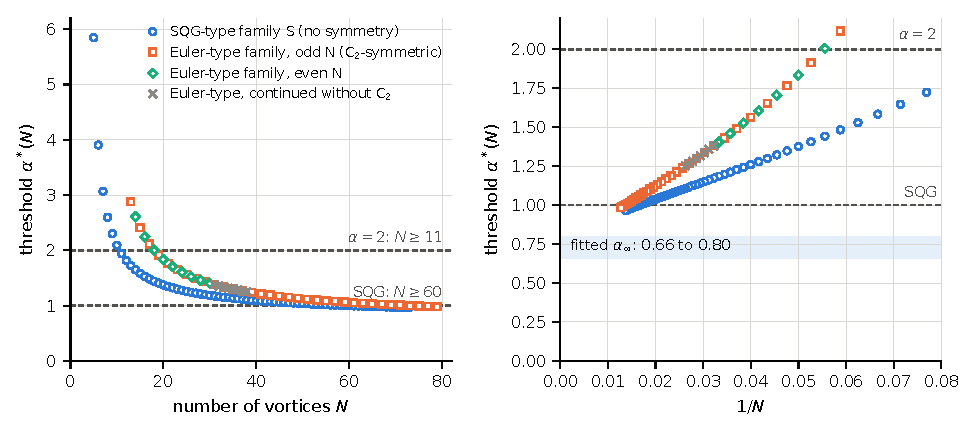
\includegraphics[width=\textwidth]{figures/phase-diagram.pdf}
  \caption{The least $\alpha$ at which $N$ vortices collapse self-similarly without rotation, along the two families $S$ and $E$ below, with the odd, even and asymmetric branches of $E$ drawn separately (numerical). Left: against $N$; the dashed lines are $\alpha = 2$ and SQG ($\alpha = 1$), crossed by the SQG-type family at $N = 11$ and $N = 60$. Right: against $1/N$; the band is the range $0.66$ to $0.80$ of the limits $\alpha_\infty$ given by the fits of Table~\ref{tab:fits}. The data are in \texttt{data/phase-diagram/alpha-star-phase-diagram.csv}.}
  \label{fig:phase}
\end{figure}

\subsection{Two families}

The \emph{SQG-type family} $S$ has one strong vortex near the collision point, one strong vortex of the opposite sign, and weak vortices of one sign, with no symmetry; the least recorded minimizers of $P$ at $\alpha = 1$ and $2$ for $N = 8$, $9$ and $10$, and the least Euler minimizer for $N = 8$, continue in $\alpha$ to its thresholds, while the least Euler minimizer for $N = 10$ reaches a larger one (Section~\ref{sec:searches}). We computed it for $5 \le N \le 73$, the new members for $N \ge 60$ by inserting a passive vortex at a stagnation point of the similarity flow and minimizing $\alpha$ again. The \emph{Euler-type family} $E$ comes from the Euler minimizers of \cite[Sect.~7]{mw2026}; its odd-$N$ thresholds are exactly $C_2$-symmetric (a central vortex and pairs $\pm w$ with equal circulations; the defect is $10^{-13}$), while the even ones are not. We extended the odd branch to $N = 79$ with the symmetric system reduced to the fixed-point set of the symmetry, and at all $34$ odd thresholds from $N = 13$ to $79$ the reduced Hessian in the full space is positive definite, so the symmetric points are strict local minima of $\alpha$ on $Z$ without the symmetry imposed. A continuation of $E$ from $N = 30$ without the symmetry gives eight more points ($31 \le N \le 38$), slightly below the odd branch at odd $N$.

The thresholds are shown in Figure~\ref{fig:phase}. Along both families $\alpha^*(N)$ decreases strictly with $N$, and $S$ is the lowest family at every $N$ where another was computed. The least $N$ with a collapse without rotation, along these families, is given in Table~\ref{tab:leastN}. For $\alpha = 2$ the values are $\alpha^*(9) = 2.3000208434$, $\alpha^*(10) = 2.0913751011$ and $\alpha^*(11) = 1.9372878365$, so eleven is the least number along $S$, in agreement with the certified collapse of \cite[Theorem~5(a)]{mw2026}. For SQG, $S$ crosses $\alpha = 1$ between $N = 59$ ($1.00246$) and $N = 60$ ($0.99921$), in agreement with \cite[Theorem~5(b)]{mw2026}, and the odd branch of $E$ crosses it between $N = 73$ ($1.00246$) and $N = 75$ ($0.99543$), so it also gives SQG collapses without rotation, $C_2$-symmetric ones, from $N = 75$. For $N > 73$ only that branch was computed. The least values computed are $0.96443$ ($S$, $N = 73$) and $0.98242$ ($E$, $N = 79$).

\begin{table}[t]
\centering
\small
\begin{tabular}{@{}lccccccccc@{}}
\toprule
$\alpha$ & $6$ & $5$ & $4$ & $3$ & $2.5$ & $2$ & $1.5$ & $1.2$ & $1$ \\
least $N$ & $5$ & $6$ & $6$ & $8$ & $9$ & $11$ & $17$ & $29$ & $60$ \\
\bottomrule
\end{tabular}
\caption{The least number of vortices with a self-similar collapse without rotation, along the families of Figure~\ref{fig:phase} (numerical; all from the family $S$).}\label{tab:leastN}
\end{table}

\subsection{The searches at \texorpdfstring{$\alpha = 2$}{alpha = 2} and at four vortices}\label{sec:searches}

Whether ten vortices can collapse without rotation at $\alpha = 2$ is not settled by one family, so we searched further. Of the nineteen recorded local minima of $P$ for $N = 8$, $9$ and $10$ at $\alpha = 0$, $1$ and $2$, eighteen were continued in $\alpha$ up to $P = 0$, followed by the minimization of $\alpha$ on $Z$; for the nineteenth, the third Euler minimum for $N = 8$, the continuation failed. Each of the eighteen ends at the threshold of $S$ for its $N$ ($2.5993690531$, $2.3000208434$ and $2.0913751011$) or at a larger value ($8.0863308796$ for $N = 8$, $5.7554694090$ and $5.2557582423$ for $N = 9$, $4.4051046186$ for $N = 10$). The least Euler minimizer for $N = 9$, $P = 0.6592598630\ldots$ \cite[Sect.~7]{mw2026}, was not among them. A random walk on $Z$ with large perturbations of positions, circulations and signs, each step followed by the minimization of $\alpha$, made $5352$ attempts with $323$ landings for $N = 9$ and $5221$ attempts with $277$ landings for $N = 10$, and found no local minimum of $\alpha$ below $2.3000208434$ and $2.0913751011$. A perturbation search for the least $P$ at $\alpha = 2$ ($1110$ attempts and $358$ landings for $N = 9$, $652$ and $191$ for $N = 10$) found the least values $0.0675758057$ and $0.0237078013$, and no point with $P = 0$. Driving the circulation of one vortex of the $\alpha = 2$, $N = 11$ collapse to zero while minimizing $\alpha$ ends, for each of the nine weak vortices, at $2.0913751011$, the ten-vortex threshold of $S$; for the strong vortex of opposite sign the homotopy did not converge, and no record of it is stored. Reduced $C_2$-symmetric systems give no lower thresholds: the least values found are $5.7555$ ($N = 9$, a center and four pairs), $4.9340$ ($N = 10$, five pairs), $3.7369$ ($N = 11$), $3.3600$ ($N = 12$) and $2.8803$ ($N = 13$). This is evidence, not a proof, that ten vortices cannot collapse without rotation at $\alpha = 2$.

For four vortices no clean threshold exists along the families we followed: the $\alpha = 2$ four-vortex minimum continues upward, $P = 0.207$ at $\alpha = 5$ and $0.069$ at $\alpha = 10$, and reaches $P = 0$ near $\alpha = 14.63$, but there three circulations are $10^{-6}$ to $6.5 \cdot 10^{-6}$ times the fourth: a strong vortex with near-passive companions. Three vortices cannot collapse without rotation for any $\alpha > -2$ \cite[Theorem~2]{mw2026}.

\subsection{The limit of many vortices}

For $20 \le N \le 50$ the decrements of $S$ are close to $11/N^2$ ($N^2|\alpha^*(N + 1) - \alpha^*(N)|$ lies between $11.03$ and $11.8$), which suggests $\alpha^*(N) \approx \alpha_\infty + 11/N$. This law does not hold: $N^2|\alpha^*(N + 1) - \alpha^*(N)|$ has its least value $11.03$ at $N = 35$ and rises to $11.9$ at $N = 72$, and the local exponent $p$ of $\alpha^* \approx a + bN^{-p}$ falls steadily, from $1.06$ at $N = 30$ to $0.90$ at $N = 48$ and $0.82$ at $N = 66$, so the approach is slower than $1/N$. Along the odd branch of $E$ the same quantity stops falling at $19.24$ near $N = 69$ and turns up. Table~\ref{tab:fits} fits five forms to the tails of both families, over three windows each. Every fit with $\alpha_\infty$ free gives a positive limit, between $0.677$ and $0.800$ for $S$ and between $0.656$ and $0.766$ for $E$: the form $a + b/(\ln N)^q$, which follows the drifting exponent, gives $0.66$ to $0.68$, the polynomial and power forms $0.72$ to $0.80$. Fits that force $\alpha_\infty = 0$ have a root-mean-square residual $30$ to $530$ times that of the same form with $\alpha_\infty$ free, and $130$ to $3400$ times that of the best free fit in the window.

\begin{table}[t]
\centering
\small
\renewcommand{\arraystretch}{1.12}
\begin{tabular}{@{}llrrrr@{}}
\toprule
family & form & \multicolumn{2}{c}{$N \ge 56$ ($S$), $N \ge 63$ ($E$)} & \multicolumn{2}{c}{$N \ge 33$ ($S$), $N \ge 40$ ($E$)} \\
 & & $\alpha_\infty$ & rms & $\alpha_\infty$ & rms \\
\midrule
$S$ & $a + b/N + c/N^2$ & $0.789$ & $5.4 \cdot 10^{-6}$ & $0.800$ & $1.5 \cdot 10^{-4}$ \\
$S$ & $a + b/N + c/N^2 + d/N^3$ & $0.776$ & $2.3 \cdot 10^{-7}$ & $0.785$ & $1.8 \cdot 10^{-5}$ \\
$S$ & $a + bN^{-p}$ & $0.767$ & $2.9 \cdot 10^{-6}$ & $0.787$ & $1.1 \cdot 10^{-4}$ \\
$S$ & $a + b/(\ln N)^q$ & $0.677$ & $4.0 \cdot 10^{-7}$ & $0.684$ & $2.1 \cdot 10^{-5}$ \\
$S$ & $b/(\ln N)^q$, $\alpha_\infty = 0$ forced & $0$ & $2.1 \cdot 10^{-4}$ & $0$ & $2.4 \cdot 10^{-3}$ \\
$E$ & $a + b/N + c/N^2 + d/N^3$ & $0.724$ & $1.4 \cdot 10^{-7}$ & $0.731$ & $8.9 \cdot 10^{-6}$ \\
$E$ & $a + b/(\ln N)^q$ & $0.656$ & $1.4 \cdot 10^{-6}$ & $0.670$ & $5.2 \cdot 10^{-5}$ \\
$E$ & $b/(\ln N)^q$, $\alpha_\infty = 0$ forced & $0$ & $3.2 \cdot 10^{-4}$ & $0$ & $3.2 \cdot 10^{-3}$ \\
\bottomrule
\end{tabular}
\caption{Fits of the thresholds of Figure~\ref{fig:phase} over trailing windows (numerical; a selection; all forms and a middle window are in \texttt{data/phase-diagram/alpha-inf-fits.json}).}\label{tab:fits}
\end{table}

This is consistent with no Euler collapse without rotation along these families. It says nothing about other families, and an approach slower than any power of $\ln N$ is not excluded by $N \le 79$. Since the first-order system of each threshold is square and nondegenerate, the interval Newton (Krawczyk) method used in \cite[Sect.~8]{mw2026} could certify any $\alpha^*(N)$ rigorously; we have not done so.

\section{Structure and stability of the collapses without rotation}\label{sec:structure}

\subsection{No mirror symmetry}

The following observation is elementary; we record it because it rules out a natural ansatz for collapses, with or without rotation.

\begin{proposition}\label{prop:mirror}
Let $\alpha$ be real and consider a self-similar collapse of $N \ge 2$ point vortices under \eqref{eq:alpha} in which all circulations and their sum are nonzero. No reflection of the plane maps the configuration onto itself, either with every circulation kept or with every circulation reversed.
\end{proposition}

\begin{proof}
Suppose a reflection $\sigma$ maps the configuration onto itself, with a permutation $\pi$ such that $\sigma(z_j) = z_{\pi(j)}$. If every circulation is reversed, $\Gamma_{\pi(j)} = -\Gamma_j$, then $\sum_j\Gamma_j = \sum_j\Gamma_{\pi(j)} = -\sum_j\Gamma_j$, so the total circulation vanishes, contrary to the hypothesis. Suppose every circulation is kept, $\Gamma_{\pi(j)} = \Gamma_j$. Then $\sigma$ fixes the center of vorticity, so after a translation and a rotation, under which \eqref{eq:alpha} is equivariant and $\kappa$ does not change, $z_c = 0$ and $\sigma(z) = \bar z$. The right side of \eqref{eq:alpha} satisfies $V_j(\bar z_1, \ldots, \bar z_N) = -\overline{V_j(z_1, \ldots, z_N)}$ for real circulations: the mirror image of a motion, run backwards, is a motion. Hence $V_{\pi(j)} = -\overline{V_j}$. The collapse gives $V_j = \kappa z_j$ and $V_{\pi(j)} = \kappa z_{\pi(j)} = \kappa\bar z_j$, so $\kappa\bar z_j = -\bar\kappa\bar z_j$ for every $j$, and since some $z_j \ne 0$, $\re\kappa = 0$, contrary to $\re\kappa < 0$.
\end{proof}

Rotational symmetry is allowed: the odd branch of $E$ in Section~\ref{sec:phase} is $C_2$-symmetric. By Proposition~\ref{prop:mirror} no member of the families of \cite[Theorem~5]{mw2026} is mirror symmetric; \texttt{verify\_\allowbreak family\_\allowbreak structure.py} checks the time-reversal identity on random configurations for $\alpha = 0$, $0.5$, $1$ and $2$, and that the mirror image of the $\alpha = 2$ collapse expands with $2\pi\kappa' = 1$.

\subsection{The nine-parameter family at \texorpdfstring{$\alpha = 2$}{alpha = 2}}\label{sec:family}

The rest of this section is numerical (binary64). At the eleven-vortex collapse of \cite[Theorem~5(a)]{mw2026}, with the rotation and the scale fixed and $2\pi\kappa = -1$, the $22$ equations have full rank in $31$ unknowns (the ratio of the smallest to the largest singular value is $7.3 \cdot 10^{-4}$), so the collapses without rotation form a manifold of dimension nine there. We continued along both signs of each of the nine tangent directions for $300$ steps, to arclengths $1.9$ to $3.9$ relative to the size of the configuration: no collision (the closest pair stays above $0.045$ of the size), no vanishing circulation and no loss of rank occurs, and the sign pattern, one strong vortex, one of the opposite sign and nine weak vortices of the sign of the strong one, never changes, while the ratio of the largest to the smallest circulation varies from $17$ to $153$.

The family has no $C_5$-symmetric member. Eleven vortices with $C_5$ symmetry form two regular pentagons and a central vortex; for two $n$-gons at radii $1$ and $\rho$, relative rotation $\theta$ and a central vortex, equal radial rates force the circulation $-1/\rho^2$ on the second ring, the central circulation enters linearly, and collapse without rotation reduces to one scalar equation $F(\rho, \theta) = 0$. On a $200 \times 200$ grid, $0.05 \le \rho \le 20$, $0 < \theta < 2\pi/n$, $F$ has one sign for $n = 2$, $3$ and $5$ at $\alpha = 1$ and $2$, with $|F|$ at least $0.03$ times its natural scale, so the scan finds no collapse without rotation of this form for five, seven or eleven vortices at these $\alpha$ with $0.05 \le \rho \le 20$; a grid does not exclude a zero of $F$ between its points, and we have not bounded $F$ rigorously. $C_2$-symmetric collapses without rotation of eleven vortices (a center and five pairs) exist, but the least $\alpha$ found for them is $3.7369117731 > 2$ (Section~\ref{sec:searches}). We found no simplest member: minimizing the spread of the nine weak circulations along the family stalls with circulations that still differ by a factor $1.32$.

\subsection{Linear stability}\label{sec:stability}

In similarity variables $z = \rho(t)\zeta$, $d\tau = \rho^{-2\beta}dt$ with $\beta = 1 + \alpha/2$, a self-similar collapse is a fixed point of $d\zeta/d\tau = V(\zeta) - \kappa\zeta$. With the circulations held fixed and $2\pi\kappa = -1$, a mode of the linearization with exponent $k$ (the real part of an eigenvalue of the Jacobian of $2\pi V(\zeta) + \zeta$) grows relative to the size $r$ of the configuration like $r^{-k}$. The Jacobian of $2\pi V$ is a Hamiltonian matrix with respect to the symplectic form weighted by the circulations, so its eigenvalues come in pairs $\pm\mu$ and the exponents $k = 1 + \re\mu$ in pairs with $k + k' = 2$, and six of them, $0$, $2\beta$, $1$, $1$, $2$ and $-\alpha$, belong to the symmetries; both facts hold to $10^{-12}$ and $4 \cdot 10^{-11}$ in the computation and check it. For the eleven vortices at $\alpha = 2$, $8$ of the $16$ shape modes are unstable, all real, with $k$ from $8.43$ to $258.15$; for the sixty SQG vortices, $57$ of the $114$ shape modes are unstable, all real, with $k$ from $5.04$ to $4273.65$.

Table~\ref{tab:stability} shows direct integrations (the DOP853 method with relative tolerance $10^{-13}$, which conserves the Hamiltonian to $3 \cdot 10^{-10}$, the impulse to $10^{-14}$ and the angular impulse to $10^{-13}$). A random perturbation of relative size $10^{-6}$ grown at the largest exponent alone reaches $10^{-2}$ at the size $10^{-4/k_{\max}}$, that is $0.965$ ($\alpha = 2$) and $0.998$ (SQG); the perturbed motions depart from the self-similar collapse, by a shape deviation of $10^{-2}$, at sizes $0.952$ to $0.956$ and $0.991$ to $0.992$, having turned by less than $10^{-4}$ rad. After departure the configuration deforms and turns (by up to $0.34$ and $0.23$ rad in the window), never gets below $0.828$ ($\alpha = 2$) and $0.887$ (SQG) of its initial size, and no close pair forms. Even unperturbed, the binary64 integrations depart at sizes $0.882$ and $0.983$ from round-off alone, so a direct simulation cannot exhibit these collapses. Lewkowicz and Kudela found the same sensitivity for a seven-vortex Euler collapse, where the scale reached before departure grows with the working precision \cite{lk2015}, without computing exponents.

\begin{table}[t]
\centering
\small
\renewcommand{\arraystretch}{1.12}
\begin{tabular}{@{}llrrrrr@{}}
\toprule
collapse & perturbation & \multicolumn{2}{c}{departure} & rotation before & least size & closest pair \\
 & & size & $t/t_c$ & departure (rad) & ($t/t_c$) & $/R_0$ \\
\midrule
$\alpha = 2$, $N = 11$ & none & $0.8819$ & $0.395$ & $4 \cdot 10^{-5}$ & $0.796$ ($0.99$) & $0.075$ \\
 & $10^{-6}$, seed 1 & $0.9524$ & $0.177$ & $4 \cdot 10^{-5}$ & $0.851$ ($0.59$) & $0.085$ \\
 & $10^{-6}$, seed 2 & $0.9529$ & $0.175$ & $2 \cdot 10^{-6}$ & $0.828$ ($0.61$) & $0.092$ \\
 & $10^{-6}$, seed 3 & $0.9558$ & $0.165$ & $2 \cdot 10^{-5}$ & $0.859$ ($0.55$) & $0.095$ \\
SQG, $N = 60$ & none & $0.9834$ & $0.049$ & $8 \cdot 10^{-5}$ & $0.895$ ($0.41$) & $0.0064$ \\
 & $10^{-6}$, seed 1 & $0.9908$ & $0.027$ & $7 \cdot 10^{-5}$ & $0.901$ ($0.47$) & $0.0061$ \\
 & $10^{-6}$, seed 2 & $0.9915$ & $0.025$ & $7 \cdot 10^{-5}$ & $0.887$ ($1.20$) & $0.0059$ \\
 & $10^{-6}$, seed 3 & $0.9915$ & $0.025$ & $6 \cdot 10^{-5}$ & $0.904$ ($0.50$) & $0.0050$ \\
\bottomrule
\end{tabular}
\caption{Direct integration of the two collapses without rotation of \cite[Theorem~5]{mw2026} to $1.5\,t_c$ ($\alpha = 2$) and $1.2\,t_c$ (SQG), with and without a random perturbation of the positions of relative size $10^{-6}$ (\texttt{verify\_\allowbreak stability.py}; numerical). Sizes are relative to the initial size $R_0$; the SQG run with seed 2 is at its least size when the window ends.}\label{tab:stability}
\end{table}

\section{The continuum limit}\label{sec:continuum}

Everything in this section is numerical, in high-precision arithmetic. O'Neil \cite{oneil2010} gave numerical evidence for collapsing vortex sheets accompanied by point vortices. He approximated each sheet by $50$ to $300$ identical point vortices and solved the point-vortex collapse equations by Newton's method. For a point vortex of circulation $-1$ and a sheet of circulation $2$ he computed collapses for several values of his ratio $\beta/\alpha$, which in our notation have $P = 1$, $5/3$ and $5$ \cite[Figs.~1, 2]{oneil2010}. He also computed configurations with two negative point vortices, among them an S-shaped sheet with point vortices of circulations $-1$ and $-0.98$ on either side, collapsing with $P = 1/2$ \cite[Fig.~3]{oneil2010}; its discretization is itself a self-similar collapse of $102$ Euler point vortices with $P = 1/2$. The continuum form of $\sum_{i<j}\Gamma_i\Gamma_j = 0$ used below is a case of his necessary condition \cite[Eq.~(6a)]{oneil2010}. The configurations of this section are of the type of his Fig.~3; he did not minimize $P$ or solve the continuous equations directly. What is new here, as far as we know, is the direct solution of the continuous equations with a spectral method and its convergence, the local minimum $P_\infty$ of the winding along the family, and its agreement with the finite minimizers of \cite[Sect.~7]{mw2026}. Kudela \cite{kudela2021} observed that in numerical self-similar collapses of fifty vortices with one, two or four strong vortices the weak vortices line up on arcs, which he calls vortex sheets.

In the two-arm family of Euler minimizers of \cite[Sect.~7]{mw2026}, a vortex at the center and two arms of weak positive vortices carry two negative vortices, and $P$ decreases with $N$ towards about $0.47736$. As $N$ grows, the weak vortices of each arm approach a curve with a smooth circulation density. We model the limit by a point-symmetric vortex sheet $z(x)$, $-1 \le x \le 1$, with $z(-x) = -z(x)$, $|dz/dx| = L$ constant (so $x$ is proportional to arclength) and the tip $z(1) = 1$, carrying the circulation $g(x)\,dx$ with $g(x) = \sqrt{1 - x^2}\,h(x)$, together with two point vortices of circulation $-1$ at $\pm z_n$. Self-similar collapse requires
\begin{equation}\label{eq:sheet}
  \mathrm{PV}\!\!\int_{-1}^{1} \frac{g(t)\,dt}{z(x) - z(t)} - \frac{1}{z(x) - z_n} - \frac{1}{z(x) + z_n} = \Lambda\,\overline{z(x)} \quad (|x| < 1), \qquad \int_{-1}^{1} \frac{g(t)\,dt}{z_n - z(t)} - \frac{1}{2z_n} = \Lambda\,\overline{z_n},
\end{equation}
the principal-value Birkhoff--Rott integral on the sheet and the velocity at the point vortex, with $\Lambda$ as in \eqref{eq:Lambda} and $P = \re\Lambda/(-2\im\Lambda)$. The continuum form of $\sum_{i<j}\Gamma_i\Gamma_j = 0$, with the sheet of total circulation $\Sigma$ contributing $\Sigma^2/2$ from its own pairs, is $1 - 2\Sigma + \Sigma^2/2 = 0$ \cite[Eq.~(6a)]{oneil2010}, whose roots are $2 \pm \sqrt{2}$.

We discretize the tangent angle of the sheet and $h$ as even Chebyshev series of $m$ terms each, evaluate the principal-value integral by Gauss--Chebyshev quadrature of the second kind with $n$ nodes, collocate at the positive zeros of the Chebyshev polynomial $T_{n+1}$, and solve the overdetermined collocation system in the least-squares sense, so that its residual measures the truncation error. The solutions form a one-parameter family, and we minimize $P$ along it. The solutions were refined by Newton steps with a binary64 Jacobian and residuals evaluated in ball arithmetic (Arb, through python-flint) at $192$ and $256$ bits; no enclosure of a solution is proved, and the digits below are not certified. They converge exponentially in $m$ (Table~\ref{tab:continuum}): the residual falls from $3.7 \cdot 10^{-18}$ at $m = 64$ to $7.6 \cdot 10^{-39}$ at $m = 140$, the values of $P$ at $m = 100$ and $m = 120$ differ from that at $m = 140$ by $8.3 \cdot 10^{-35}$ and $1.3 \cdot 10^{-40}$, a factor $6 \cdot 10^5$ per twenty terms, and so, if that rate, estimated from these few resolutions, persists,
\[
  P_\infty = 0.4773635336916120248430486309060121246263\ldots
\]
to forty digits. At the solution the sheet carries $2 + \sqrt{2}$, each arm $1 + 1/\sqrt{2}$, and the angular impulse vanishes, to $10^{-43}$. Independently of the collocation, the continuous equations \eqref{eq:sheet} hold between the collocation points to $2 \cdot 10^{-13}$, with the principal value computed by subtracting the singularity and adaptive quadrature at forty digits from the stored coefficients rounded to binary64. Along the family, $dP/dc = 0$ and $d^2P/dc^2 = 0.1096 > 0$ in the family coordinate $c$, so $P_\infty$ is a local minimum along it; we restricted the density to vanish like a square root at the tips, and whether another tip behavior gives a smaller $P$ is not settled here.

\begin{table}[t]
\centering
\small
\renewcommand{\arraystretch}{1.12}
\begin{tabular}{@{}rrrlr@{}}
\toprule
$m$ & $n$ & bits & $P$ & collocation residual \\
\midrule
$64$ & $384$ & $192$ & $0.47736353369161202484304865\ldots$ & $3.7 \cdot 10^{-18}$ \\
$80$ & $480$ & $192$ & $0.4773635336916120248430486309556\ldots$ & $1.7 \cdot 10^{-22}$ \\
$100$ & $800$ & $256$ & $0.47736353369161202484304863090601204\ldots$ & $7.0 \cdot 10^{-28}$ \\
$120$ & $960$ & $256$ & $0.4773635336916120248430486309060121246264\ldots$ & $2.5 \cdot 10^{-33}$ \\
$140$ & $840$ & $256$ & $0.4773635336916120248430486309060121246263\ldots$ & $7.6 \cdot 10^{-39}$ \\
\bottomrule
\end{tabular}
\caption{The local minimum of the winding along the family of solutions of the continuum model \eqref{eq:sheet} at five resolutions (numerical; $m$ Chebyshev terms per unknown function, $n$ quadrature nodes; \texttt{verify\_\allowbreak continuum\_\allowbreak limit.py}).}\label{tab:continuum}
\end{table}

The limit agrees with the finite family: a fit $P(N) = a + b/N + \cdots + e/N^4$ to the $31$ members with $N \ge 301$ of \cite[Sect.~7]{mw2026}, whose values are stored to thirteen digits, gives $a = P_\infty - 9 \cdot 10^{-13}$, and fixing $a = P_\infty$ leaves the residual at the rounding level, $2.7 \cdot 10^{-14}$; cubic Richardson extrapolation in $1/N$ through $N = 101$, $203$, $403$ and $603$ gives $0.477363529$. In the limit the sheet has half-length $L = 1.0306552905$, the point vortices sit at $\pm(0.7678760388 + 0.1405296657\,i)$ and $\Lambda = 4.2243187321 - 4.4246349312\,i$; the circulation per unit length is $1.3190$ at the center and largest, $2.3308$, at $0.707$ of the half-length, and it vanishes like a square root at the tips; the tangent of the sheet turns from $9.32^\circ$ at the center to $33.98^\circ$ at the tip. We have found no closed form for $P_\infty$: with forty digits, no algebraic relation of degree at most five with integer coefficients up to $10^6$ holds for $P_\infty$, $P_\infty^2$, $1/P_\infty$, $\arctan(2P_\infty)/\pi$ or $4P_\infty^2 + 1$, and no integer relation with coefficients up to $10^6$ connects $P_\infty$, $P_\infty^2$ or $1/P_\infty$ with $1$ and three or four of $\sqrt{2}$, $\sqrt{3}$, $\pi$, $\ln 2$, $\ln 3$, $e$ and $\ln(1 + \sqrt{2})$; at these sizes a relation found by chance would need larger coefficients.

\section{Numerical verification}\label{sec:numerics}

Table~\ref{tab:checks} lists the programs. Each prints every check with its result, stops with an error if one fails, and writes its report to \texttt{data/}; under Python~3.11 with the package versions of \texttt{code/requirements.txt} each runs in about two minutes or less, the stability program in its full form in two and a half. The programs \texttt{verify\_\allowbreak phase\_\allowbreak diagram.py}, \texttt{verify\_\allowbreak family\_\allowbreak structure.py} and \texttt{verify\_\allowbreak stability.py} share the module \texttt{collapse\_\allowbreak core.py} (the law \eqref{eq:alpha}, its analytic Jacobian, Newton's method and the first-order system of the minimization of $\alpha$), and \texttt{verify\_\allowbreak continuum\_\allowbreak limit.py} uses \texttt{continuum\_\allowbreak model.py} (the discretization, in binary64) and \texttt{continuum\_\allowbreak arb.py} (the same residual in Arb, and the refinement, which also runs as a program). The convergence checks of \texttt{verify\_\allowbreak cluster\_\allowbreak collapses.py} require the error of each asymptotic statement to fall by a factor of at least five per decade of $\gamma$, instead of fixed tolerances. The inputs taken from \cite{mw2026}, the two certified collapses without rotation, the four-vortex minimum and the two-arm family, are copied into \texttt{data/}.

{\small
\renewcommand{\arraystretch}{1.2}
\begin{longtable}{|>{\raggedright\arraybackslash}p{0.33\textwidth}|>{\raggedright\arraybackslash}p{0.47\textwidth}|>{\raggedleft\arraybackslash}p{0.09\textwidth}|}
\caption{The verification programs, what they check, and the number of checks.}\label{tab:checks}\\
  \hline
  \textbf{Program} & \textbf{What it checks} & \textbf{Checks} \\ \hline
  \endfirsthead
  \hline
  \textbf{Program} & \textbf{What it checks} & \textbf{Checks} \\ \hline
  \endhead
  \texttt{verify\_\allowbreak cluster\_\allowbreak identities.py} & Every identity in the proof of Theorem~\ref{thm:clusters} and of Section~\ref{sec:formal}, exactly (SymPy): (I1), (I2), the expansions behind \eqref{eq:A} and \eqref{eq:B}, \eqref{eq:trans}, \eqref{eq:nu}, \eqref{eq:imp}, the constants of (d) for every $n$, Remark~\ref{rem:harmonic}, the formal expansion and the triple slope; negative controls & $62$ \\ \hline
  \texttt{verify\_\allowbreak cluster\_\allowbreak remainders.py} & The remainders of \eqref{eq:A}, \eqref{eq:B} and \eqref{eq:W} on 150 random configurations of $\K(n, 0.3)$, $\gamma = 10^{-2}$ to $10^{-7}$, bounded after division by their order, and a control that grows like $1/\gamma$; the constants of Step~1 and of (d) on 400 random configurations with up to 40 weak vortices & $8$ \\ \hline
  \texttt{verify\_\allowbreak cluster\_\allowbreak collapses.py} & Collapses computed at fifty digits for eight cluster arrangements at $\gamma = 10^{-2}, 10^{-3}, 10^{-4}$ (Table~\ref{tab:clusters}), with convergence tests of \eqref{eq:formal} and of part (b); singletons and (d) on rings with a strong center; the controls of Remark~\ref{rem:class} and Section~\ref{sec:formal}. About two minutes (\texttt{-{}-quick}: one minute, 72 checks) & $90$ \\ \hline
  \texttt{verify\_\allowbreak triple\_\allowbreak branch.py} & Theorem~\ref{thm:triple} and Corollary~\ref{cor:triple}: the point at $\gamma = 0$, the closed form of $d(w_1 - w_2)$ and the slope $2\sqrt{3}\,g_1g_2g_3/S$, exactly over $\Q(t)(\omega)$; the family at forty digits for four triples and both $\omega$, checked against the Biot--Savart equations of all four vortices, with the convergence of the slope; other $y_0$; a triple with $g_1g_2g_3 > 0$; the class $\K(3, 1/2)$; controls. About ten seconds & $62$ \\ \hline
  \texttt{verify\_\allowbreak sharpness\_\allowbreak all\_\allowbreak n.py} & Lemma~\ref{lem:grow} and Corollary~\ref{cor:alln}: the pair and the triangle exactly (translation, nondegeneracy, the zeros of $R$ and the discriminant $-216$); clusters of $4$ to $15$ vortices grown by the induction from both starting clusters (binary64), and their families of Theorem~\ref{thm:cluster} at forty digits, checked against the Biot--Savart equations of all vortices; controls; optionally a cluster of $101$ vortices. About twenty seconds (\texttt{-{}-large}: a minute) & $37$ ($40$) \\ \hline
  \texttt{verify\_\allowbreak cluster\_\allowbreak stored.py} & The 21 stored collapses rechecked with separate code at sixty digits: least-squares $\kappa$ over all vortices, both invariants, $P$, membership in $\K(n, c)$ with $c \ge 0.37$, and the exact net circulation of Remark~\ref{rem:harmonic} & $26$ \\ \hline
  \texttt{verify\_\allowbreak phase\_\allowbreak diagram.py} & All 120 thresholds of Figure~\ref{fig:phase} from their stored configurations: collapse without rotation, first-order conditions, reduced Hessians, $C_2$ defects; Tables~\ref{tab:leastN} and~\ref{tab:fits}; the $11/N$ law and the local exponent; the end points of the searches of Section~\ref{sec:searches} & $46$ \\ \hline
  \texttt{plot\_\allowbreak phase\_\allowbreak diagram.py} & Figure~\ref{fig:phase} from the table & \\ \hline
  \texttt{verify\_\allowbreak family\_\allowbreak structure.py} & Section~\ref{sec:family}: the dimension nine, 18 continuations, the time-reversal identity of Proposition~\ref{prop:mirror} and the mirror image, the ring reduction against Biot--Savart and its one-signed $F$, the most nearly equal weak circulations & $15$ \\ \hline
  \texttt{verify\_\allowbreak stability.py} & Section~\ref{sec:stability}: symmetry exponents, the pairing $k + k' = 2$, the unstable modes, and the eight integrations of Table~\ref{tab:stability}. Two and a half minutes (\texttt{-{}-quick}: SQG integrations to $0.08\,t_c$, 20 s, 13 checks) & $14$ \\ \hline
  \texttt{verify\_\allowbreak continuum\_\allowbreak limit.py} & Section~\ref{sec:continuum}: convergence in $m$, the two finest solutions recomputed in Arb, $\Sigma = 2 + \sqrt{2}$ (SymPy), the residual between collocation points, local minimality, the finite family, the shape, and the closed-form searches & $13$ \\ \hline
  \texttt{continuum\_\allowbreak arb.py} & Run as a program: the refinement of Section~\ref{sec:continuum} at $m = 64$, $n = 384$ from sixteen digits; it reproduces the stored value to $9 \cdot 10^{-25}$, well inside that resolution's residual $3.7 \cdot 10^{-18}$ & \\ \hline
\end{longtable}
}

\section{Discussion}\label{sec:discussion}

Theorem~\ref{thm:clusters} extends \cite[Theorem~3]{mw2026} from pairs to clusters, and its proof follows the same compactness scheme; the new ingredients are the identities (I1) and (I2) of the internal field, which reduce every cluster at leading order to its net circulation $G_C$ and its dipole $D_C$, and the observation that the leading-order equations of a cluster are those of a pair with $u_j$ replaced by $q_C$. For one pair, Krishnamurthy and Stremler describe a small dipole in the field of a strong vortex \cite[Sect.~3.6, Fig.~9]{ks2018}, as the companion paper records. That a vortex pair with separation $\varepsilon$ and net circulation of order $\varepsilon^2$ behaves as a charged particle is the scaling of Drivas, Glukhovskiy and Khesin \cite[Theorem~1.1]{dgk2024}, who prove it for pairs on surfaces without a strong vortex and without collapse; our clusters have the same scaling, net circulation of order $\gamma^2$ at size $\gamma$. Leoncini, El Kettani and Ugalde \cite[Sect.~B]{leu2026} expand in the size of a small triple whose net circulation equals that of a parent vortex, the opposite case of ours, and do not discuss winding. Lydon, Nazarenko and Laurie \cite{lnl2022} study dipoles scattering on clusters of like-signed vortices. O'Neil \cite{oneil2011, oneil2013} studies relative equilibria in which point vortices form clusters, with several scaling regimes; these are relative equilibria, not collapses. In the literature we have read we have found no treatment of near-neutral clusters in a collapse, and no bound on the winding for them; Kudela's weak vortices \cite{kudela2021} are like-signed and spread along arcs, not near-neutral clusters.

For collapses without rotation with more than three vortices, the only results we know are those of \cite{mw2026}. The $\alpha$-model collapse literature we have read treats three vortices, or, as Grotto and Pappalettera \cite{gp2025} do, collapses and bursts of many vortices constructed from a three-vortex self-similar one, which are not self-similar; Badin and Barry \cite{bb2018} derive the conditions for collapse in these models. We have not found a map of the thresholds $\alpha^*(N)$ in the literature we have read; ours is numerical and covers two families only.

The linear stability of self-similar collapse is classical for three vortices; see the discussion and references in \cite[Sect.~9]{mw2026}. For more vortices, Zbarsky \cite[p.~20]{zbarsky2024} notes that stability of some self-similarly expanding system of more than three point vortices would extend his Corollary~16 to that system, and Lydon, Nazarenko and Laurie \cite[p.~39]{lnl2022} raise the stability of vortex collapse as a question; Lewkowicz and Kudela \cite{lk2015} observed the sensitivity numerically. Section~\ref{sec:stability} computes the exponents for the two collapses without rotation. By Proposition~\ref{prop:mirror} the mirror image of a collapse is an expansion with the same shape, whose exponents are those of the collapse with the sign of time reversed.

The continuum model of Section~\ref{sec:continuum} is a vortex sheet with two point vortices that shrinks self-similarly onto a point, unlike self-similar spiral sheets that roll up and grow; O'Neil \cite{oneil2010} gave the first numerical evidence for such collapsing sheets, with point vortices approximating the sheet, and the sheet-like arcs of Kudela \cite{kudela2021} are of the same kind. The minimum $P_\infty$ along the family, and the direct solution of the continuous equations, are new as far as we know.

\paragraph{Meaning and limits.} A strong vortex that gathers weak vortices into neutral-looking clusters still turns, while shrinking by the factor $10$, by nearly $(\sqrt{3}/2)\ln 100 \approx 4$ radians if the clusters are weak, whatever their number and shape; to turn less, the weak vortices must be strong enough, or organized differently, and the first way to do it, a $(+,+,-)$ triple, is the structure of the certified four-vortex minimum. Collapse without rotation needs much more: along our families it needs $\alpha > 0.96$ for up to $79$ vortices, and the thresholds do not appear to tend to the Euler value. The collapses without rotation that exist are unstable in many directions, so they are exceptional motions, not attractors. All results concern point vortices; finite cores regularize the collision.

\section{Open problems}\label{sec:open}

\begin{enumerate}
\item Can Euler vortices collapse self-similarly without rotation, for some number of vortices? Theorem~\ref{thm:clusters} excludes the regime of a strong vortex with weak tight clusters, and Section~\ref{sec:phase} finds none along two families up to $79$ vortices. For $\alpha = 0$ such a collapse is a relative equilibrium of the imaginary circulations $i\Gamma_j$ \cite[Sect.~10]{mw2026}, a characterization that might be used.
\item Is $\alpha_\infty = \lim_{N\to\infty}\alpha^*(N)$ positive, along these families or over all collapses without rotation? A proof that $\alpha^*(N)$ is bounded below by a positive constant would settle the Euler question for the families. Short of that, the thresholds $\alpha^*(N)$ can be certified by the interval methods of \cite{mw2026}.
\item Does the continuum problem \eqref{eq:sheet} have a solution, and is the local minimum $P_\infty$ of its winding a known constant? Does a sheet with another behavior at its tips, or with more point vortices, wind less?
\item Are the thresholds of Section~\ref{sec:phase} global minima, that is, are $11$ at $\alpha = 2$ and $60$ at $\alpha = 1$ the least numbers of vortices that collapse without rotation?
\item Can the expansion \eqref{eq:formal} be proved for several clusters, or for one cluster of more than three vortices (Theorem~\ref{thm:cluster} gives the family but not its first-order coefficient), and does a strong vortex with clusters whose $e_C$ are all nonpositive satisfy $P > \sqrt{3}/2$ at every small fixed $\gamma$, as pairs do \cite[Proposition~4]{mw2026}?
\end{enumerate}

\medskip
{\raggedright\noindent\textbf{Data availability.} The programs \texttt{verify\_\allowbreak cluster\_\allowbreak identities.py}, \texttt{verify\_\allowbreak cluster\_\allowbreak remainders.py}, \texttt{verify\_\allowbreak cluster\_\allowbreak collapses.py}, \texttt{verify\_\allowbreak triple\_\allowbreak branch.py}, \texttt{verify\_\allowbreak sharpness\_\allowbreak all\_\allowbreak n.py}, \texttt{verify\_\allowbreak cluster\_\allowbreak stored.py}, \texttt{verify\_\allowbreak phase\_\allowbreak diagram.py}, \texttt{verify\_\allowbreak family\_\allowbreak structure.py}, \texttt{verify\_\allowbreak stability.py} and \texttt{verify\_\allowbreak continuum\_\allowbreak limit.py}, with the modules \texttt{collapse\_\allowbreak core.py}, \texttt{continuum\_\allowbreak model.py} and \texttt{continuum\_\allowbreak arb.py}, and \texttt{plot\_\allowbreak phase\_\allowbreak diagram.py}, used for Figure~\ref{fig:phase}, and their output and inputs will be in the repository \url{https://github.com/ChaseHendrick/collapse-without-rotation}: the programs in \texttt{code/}, their inputs and output in \texttt{data/}, and the figure in \texttt{paper/figures/}.\par}

\noindent\textbf{Funding.} This research received no external funding.

\smallskip
\noindent{\footnotesize This work was prepared with AI assistance. The author takes full responsibility for its content.}

\begin{thebibliography}{17}
\small

\bibitem{art1992} H. Aref, N. Rott and H. Thomann, Gr\"obli's solution of the three-vortex problem, \emph{Annu. Rev. Fluid Mech.} \textbf{24} (1992) 1--21.

\bibitem{bb2018} G. Badin and A. M. Barry, Collapse of generalized Euler and surface quasigeostrophic point vortices, \emph{Phys. Rev. E} \textbf{98} (2018) 023110; arXiv:1805.10127.

\bibitem{dk2014} M. V. Demina and N. A. Kudryashov, Rotation, collapse, and scattering of point vortices, \emph{Theor. Comput. Fluid Dyn.} \textbf{28} (2014) 357--368; doi:10.1007/s00162-014-0319-4.

\bibitem{dgk2024} T. D. Drivas, D. Glukhovskiy and B. Khesin, Singular vortex pairs follow magnetic geodesics, \emph{Int. Math. Res. Not. IMRN} \textbf{2024} (2024) 10880--10894; doi:10.1093/imrn/rnae106; arXiv:2401.08512.

\bibitem{gp2025} F. Grotto and U. Pappalettera, Collapse and burst of generalized surface quasi-geostrophic point vortices, \emph{Nonlinearity} \textbf{38} (2025) 105020; arXiv:2505.19782.

\bibitem{mw2026} C. Hendrick, Minimal winding in the self-similar collapse of point vortices, preprint (2026); programs and data, release v2.0.0, doi:10.5281/zenodo.22963796, at \url{https://github.com/ChaseHendrick/minimal-winding}.

\bibitem{kimura1987} Y. Kimura, Similarity solution of two-dimensional point vortices, \emph{J. Phys. Soc. Jpn.} \textbf{56} (1987) 2024--2030.

\bibitem{ks2018} V. S. Krishnamurthy and M. A. Stremler, Finite-time collapse of three point vortices in the plane, \emph{Regul. Chaotic Dyn.} \textbf{23} (2018) 530--550.

\bibitem{kudela2021} H. Kudela, Collapse of $n$ point vortices, formation of the vortex sheets and transport of passive markers, \emph{Energies} \textbf{14} (2021) 943; doi:10.3390/en14040943.

\bibitem{leu2026} X. Leoncini, P. El Kettani and E. Ugalde, Intrinsic dynamical shadowing of point vortices and finite time singularities, preprint, arXiv:2609.25989 (2026).

\bibitem{lk2015} M. Lewkowicz and H. Kudela, Collapse of $n$ vortices, preprint, arXiv:1512.05116 (2015).

\bibitem{lnl2022} K. Lydon, S. V. Nazarenko and J. Laurie, Dipole dynamics in the point vortex model, \emph{J. Phys. A} \textbf{55} (2022) 385702; arXiv:2112.13365.

\bibitem{oneil1987} K. A. O'Neil, Stationary configurations of point vortices, \emph{Trans. Amer. Math. Soc.} \textbf{302} (1987) 383--425.

\bibitem{oneil2010} K. A. O'Neil, Collapse and concentration of vortex sheets in two-dimensional flow, \emph{Theor. Comput. Fluid Dyn.} \textbf{24} (2010) 39--44; doi:10.1007/s00162-009-0106-9.

\bibitem{oneil2011} K. A. O'Neil, Clustered equilibria of point vortices, \emph{Regul. Chaotic Dyn.} \textbf{16} (2011) 555--561; doi:10.1134/S1560354711060013.

\bibitem{oneil2013} K. A. O'Neil, Singular continuation of point vortex relative equilibria on the plane and sphere, \emph{Nonlinearity} \textbf{26} (2013) 777--804; doi:10.1088/0951-7715/26/3/777.

\bibitem{zbarsky2024} S. Zbarsky, Bounds on growth and impossibility of collapse for point vortex systems, preprint, arXiv:2402.07316 (2024).

\end{thebibliography}

\end{document}
